% !TEX root = FDS_Validation_Guide.tex

\chapter{Description of Experiments}

\label{Experiments_Chapter}

This chapter contains a brief description of the experiments that were used for model validation. Only enough detail is included here to provide a general understanding of the model simulations. Anyone wishing to use the experimental measurements for validation ought to consult the cited test reports or other publications for a comprehensive description.


\section{ArupFire Tunnel Fire Experiments}

Gabriele Vigne and Jimmy J\"{o}nsson of ArupFire conducted a series of fire experiments within a tunnel with a 50~m$^2$ cross section. The tunnel is located in La Ribera del Folgoso, Spain. It is approximately 6.5~m high, 8~m wide and 300~m long. Five replicate tests were conducted using a 1~m by 2~m steel pan filled with heptane on water. Near-ceiling temperatures were measured 2~m, 4~m, 6~m and 8~m from the plume centerline. The peak heat release rate was approximately 5.3~MW.


\section{ATF Corridors Experiments}

A series of eighteen experiments were conducted in a two-story structure with long hallways and a connecting stairway in the large burn room of the ATF Fire Research Laboratory in Ammendale, Maryland, in 2008~\cite{Sheppard:Corridors}. The test enclosure consisted of two 17.0~m long hallways connected by a stairway consisting of two staircases and an intermediary landing. There was a door at the opposite end of the first floor hallway, which was closed during all tests. The end of the second floor hallway was open with a soffit near the ceiling.

The walls and ceilings of the test structure were constructed of 1.2~cm gypsum wallboard. The flooring throughout the structure, including the stairwell landing floor, consisted of one layer of 1.3~cm thick cement board on one layer of 1.9~cm thick plywood supported by wood joists. The first set of stairs, which had eight risers, led from the first floor up to the landing area. The second set of stairs, which had nine risers, led from the landing area up to the second floor. The stairs were constructed of 2.5~cm thick clear pine lumber. The two set of stairs were separated by an approximately 0.42~m wide gap in the middle of the stairwell. This gap was separated from the stairs by a 0.91~m tall barrier constructed of a single piece of gypsum board. The flue space was open to the first floor.  The flue space was separated from the second floor by a 0.9~m tall barrier constructed of gypsum board. There was a metal exterior type door at the end of the first floor near the burner.  The door was closed during all experiments.

The fire source was a natural gas diffusion burner.  The burner surface was horizontal, square and 0.45~m on each side, its surface was 0.37~m above the floor, and it was filled with gravel. The burner was located near the end of the first floor away from the stairs. A diagram of the test structure is displayed in Figure~\ref{ATF Drawing}.

\begin{figure}[p]
\includegraphics[width=\textwidth]{FIGURES/ATF_Corridors/ATF_Corridors_Drawing}
\caption{Geometry of the ATF Corridors Experiments.}
\label{ATF Drawing}
\end{figure}

\section{Backward Facing Step}

A common validation experiment for CFD codes involves flow through a channel with a backward facing step. These experiments are designed to test the influence of grid resolution, inlet turbulence, wall boundary treatments, and eddy viscosity models. One set of experiments has been conducted by Jovic and Driver~\cite{JD:1994}.  A schematic view of the experiment is shown in Fig.~\ref{tunnel_drawing}. The dimensions of the channel are based on step height $h$ = 0.0098 m.  The length of the channel is $24 \, h$. The width of the channel is $4 \, h$. The height of the inlet section is $5 \, h$, and the height of the channel downstream of the step is $6 \, h$. The expansion ratio is thus 1.2.  The inlet is split into three sub-inlets to permit localized variation of inlet turbulence.  The Reynolds number of the flow is 5100, based on the free-stream velocity (7.2~m/s) and the step height.

\begin{figure}[!ht]
\includegraphics[width=\textwidth]{FIGURES/Backward_Facing_Step/tunnel_drawing}
\caption[Geometry of the Backward Facing Step experiments]{Geometry of the Backward Facing Step experiments.}
\label{tunnel_drawing}
\end{figure}


\section{Beyler Hood Experiments}

Craig Beyler performed a large number of experiments involving a variety of fuels, fire sizes, burner diameters, and burner distances beneath a hood~\cite{Beyler:Hood}.  The hood consisted of concentric cylinders separated by an air gap.  The inner cylinder was shorter than the outer and this allowed combustion products to be removed uniformly from the hood perimeter.  The exhaust gases were then analyzed to determine species concentrations. The burner could be raised and lowered with respect to the bottom edge of the hood.  Based on the published measurement uncertainties, species errors are estimated at 6~\%.  148 tests were performed with measurements made in the exhaust duct.  The fuels in those tests were as follows: 16 acetone, 11 ethanol, 13 isopropanol, 18 methanol, 51 propane, 28 propylene, and 11 toluene. Hood equivalence ratios varied from 0.2 to 1.7.  A subset of 47 tests spanning the equivalence ratio range for each fuel was simulated for validation (5, 5, 5, 5, 15, 7, and 5 respectively for the fuels mentioned above).


\section{Bouchair Solar Chimney}

To evaluate solar-induced ventilation systems in desert climates, Bouchair~\cite{Bouchair:Thesis} constructed a simple test apparatus shown in Fig.~\ref{Bouchair_Drawing}. A compartment with interior dimensions of approximately 1.6~m long, 1.8~m, and 2.0~m high had a window on one side and an air inlet slot on the other, leading into a 1.5~m wide cavity with two heating panels spanning the long dimension. The panels were heated to 10~$^\circ$C, 20~$^\circ$C, 30~$^\circ$C, or 40~$^\circ$C above ambient, drawing air through the compartment and into the thermal cavity. The mass flow rate of air through the cavity was measured. The inlet slot was either 0.1~m or 0.4~m high, and 1.4~m wide. The thermal cavity was 1.5~m wide, and the hot panels were separated by 0.1~m, 0.2~m, 0.3~m, 0.5~m, or 1.0~m. In all, there were 40 different sets of test parameters.

In addition to the results presented in this guide, simulations of this experiment were performed by Shi and Zhang~\cite{Shi:BE2016}. The objective of the simulations is to predict the mass flow rate by accurately modeling the convective heat transfer between the air and hot panels.

\begin{figure}[!ht]
\includegraphics[trim={16in 2.5in 16in 2.5in},clip,width=\textwidth]{FIGURES/Bouchair_Solar_Chimney/Bouchair_Solar_Chimney}
\caption[Geometry of the Bouchair Solar Chimney experiment]{Geometry of the Bouchair Solar Chimney experiment.}
\label{Bouchair_Drawing}
\end{figure}



\section{BRE Spray Test for Radiation Attenuation}

Murrel et al.~\cite{Murrel:1995} measured the attenuation of thermal radiation passing through a water
spray using a heat flux gauge. The radiation was produced by a heat panel, one meter square, at 900~$^\circ$C. The horizontal distance
from the radiation panel to the spray nozzle was 2 m and to the measurement point 4 m. The nozzles were positioned at
a height 0.24 m above the panel upper edge. The heat flux gauge was positioned at the line passing through the center
of the panel. The attenuation of radiation was defined as $(q_0-q_s)/q_0$, where $q_0$ is the initial radiative heat flux,
measured without a spray, and $q_s$ is the heat flux measured during the spray operation.

Experimental results are used from three full-cone type nozzles, labeled A, B and D. The opening angles of the nozzles were between 90 and 108 degrees.
The purpose of the simulation is to compare the measured and simulated attenuation of radiation at different flow conditions. The nozzles were
specified in terms of median droplet size and mean vertical velocity using PDPA measurement in a single position, 0.7 m below the nozzle. The droplet
boundary conditions were determined by assuming $d_m \propto p^{-1/3}$ and $v \propto p^{1/2}$ type of dependencies between the droplet size, speed
and pressure.

\section{Bryant Doorway Velocity Measurements}

Rodney Bryant of the Fire Research Division at NIST performed a series of velocity measurements of the gas velocity within the doorway of a standard ISO~9705 compartment for fires ranging from 34~kW to 511~kW~\cite{Bryant:FSJ2009,Bryant:EF2009,Bryant:CS2010}. A doorway served as the only vent for the enclosure. It included a jamb of 37~cm extending outward to facilitate the laser measurements. The entire compartment was elevated 0.3~m off the floor of the laboratory (see Fig.~\ref{Bryant_Drawing}). The measurements were made using both bi-directional probes and PIV (Particle Image Velocimetry). The PIV measurements only cover the
lower two-thirds of the doorway because of difficulties in seeding the hot outflow gases. The bi-directional probe measurements span the entire height of the doorway, but Bryant reports that these measurements were up to 20~\% greater than the PIV measurements in certain regions of the flow. Consequently, only the PIV data was used for comparison to the model.

\begin{figure}[ht]
\includegraphics[width=\textwidth]{FIGURES/Bryant_Doorway/Bryant_Compartment}
\caption[Geometry of Bryant's compartment]{Geometry of Bryant's compartment.}
\label{Bryant_Drawing}
\end{figure}


\section{Cable Response to Live Fire -- CAROLFIRE}

CAROLFIRE was a project sponsored by the U.S.~Nuclear Regulatory Commission to study the thermal response and functional behavior of electrical cables~\cite{CAROLFIRE}. The primary objective of CAROLFIRE was to characterize the various modes of electrical failure (e.g., hot shorts, shorts to ground) within bundles of power, control and instrument cables. A secondary objective of the project was to develop a simple model to predict \underline{th}ermally-\underline{i}nduced \underline{e}lectrical \underline{f}ailure (THIEF). The measurements used for these purposes were conducted at Sandia National Laboratories and are described in Volume II of the CAROLFIRE test report. In brief, there were two series of experiments. The first were conducted within a heated cylindrical enclosure. Single and bundled cables were exposed to various heat fluxes and the electrical failure modes recorded. The second series of experiments involved cables within trays in a semi-enclosed space under which a gas-fueled burner created a hot layer to force cable failure. Only results from the first series are used here.

Petra Andersson and Patrick Van Hees of the Swedish National Testing and Research Institute (SP) proposed that a cable's thermally-induced electrical failure can be predicted via a one-dimensional heat transfer calculation, under the assumption that the cable can be treated as a homogenous cylinder~\cite{Andersson:2005}. Their results for PVC cables were encouraging and suggested that the simplification of the analysis is reasonable and that it should extend to other types of cables. The assumptions underlying the THIEF model are as follows:
\begin{enumerate}
\item The heat penetration into a cable of circular cross section is primarily in the radial direction.
\item The cable is homogeneous in composition. In reality, a cable is constructed of several different types of polymeric materials, cellulosic fillers, and a conducting metal, most often copper.
\item The thermal conductivity, specific heat, and density of the assumed homogeneous cable are independent of temperature. In reality, both the thermal conductivity and specific heat of polymers are temperature-dependent, but this information is not easily obtained from manufacturers.
\item It is assumed that no decomposition reactions occur within the cable during its heating, and ignition and burning are not considered in the model. In fact, thermoplastic cables melt, thermosets form a char layer, and both release volatile gases up to and beyond the point of electrical failure.
\item Electrical failure occurs when the temperature just inside the cable jacket reaches an experimentally determined value.
\end{enumerate}


\section{CSIRO Grassland Fires}

In July and August of 1986, the Commonwealth Scientific and Industrial Research Organisation (CSIRO) of Australia conducted controlled grassland fire experiments near Darwin, Northern Territory~\cite{Cheney:IJWF1993}. July and August are in the middle of the dry season when the grasses are fully cured (dried) and the weather is warm and dry. The experiments were conducted on flat plots measuring 100~m by 100~m, 200~m by 200~m, or 200~m by 300~m. Two of these experiments were simulated with FDS by Mell~et~al.~\cite{Mell:IJWF2007} and are included in this guide. Case~C064 was conducted on a 100~m by 100~m plot of kerosene grass ({\it Eriachne burkittii}); Case~F19 was conducted on a 200~m by 200~m plot of kangaroo grass ({\it Themeda australis}).


\section{Cup Burner Experiments}

The cup-burner is a widely used experimental apparatus for studying the effectiveness of flame extinguishing agents. The test is designed to determine the effectiveness of various extinguishing agents. Typically, these experiments feature a steady fuel-air coflow diffusion flame that is established above the cup. The extinguishing agent is gradually introduced into the air stream to determine the minimum concentration of the agent that leads to lift off. Two experimental data sets are examined: methane (CH$_4$) - air coflow~\cite{Takahashi:2007} and n-heptane (C$_7$H$_{16}$) - air coflow~\cite{Moore:1996}. The extinguishing agents of interest are argon (Ar), carbon dioxide (CO$_2$), helium (He), and nitrogen (N$_2$).

\section{DelCo Trainer Experiments}
\label{DelCo_Description}

The NIST Fire Fighting Technology Group conducted a series of experiments in two structures of similar design located at the Delaware County (``DelCo'') Emergency Services Training Center in Sharon Hill, Pennsylvania~\cite{DelCo_TN}. Three propane burners were used to provide the fire source for all experiments, and various sensors were used to collect gas temperature, gas velocity, heat flux, and gas concentration measurements throughout the structure.

The single level structure was instrumented with five bare-bead thermocouple arrays and two gas sample inlet pipes at the locations shown in Fig.~\ref{fig:east_instrumentation}.
\begin{figure}[!ht]
\includegraphics[width=\columnwidth]{FIGURES/DelCo_Trainers/East_Structure_Dimensioned_Instrumentation}
\caption[Instrumentation of the single level DelCo training structure]{Instrumentation of the single level DelCo training structure. The thermocouple arrays are denoted by crossed circles and the gas sampling measurement locations are denoted by hexagons at locations A1 and A4. The burner is denoted by three cross-hatched squares.}
\label{fig:east_instrumentation}
\end{figure}
Both floors of the two level structure were instrumented with three bare-bead thermocouple arrays and one gas sample inlet pipe at the locations shown in Fig.~\ref{fig:west_instrumentation}.
\begin{figure}[p]
\includegraphics[width=0.94\columnwidth]{FIGURES/DelCo_Trainers/West_Structure_2nd_Floor_Dimensioned_Instrumentation}
\\~\\
\includegraphics[width=\columnwidth]{FIGURES/DelCo_Trainers/West_Structure_1st_Floor_Dimensioned_Instrumentation}
\caption[Instrumentation of the two level DelCo training structure]{Instrumentation of the second floor (top) and first floor (bottom) of the two level DelCo training structure. The thermocouple arrays are denoted by crossed circles and the gas sampling measurement locations are denoted by hexagons at locations A1 and A10. The burner is denoted by three cross-hatched squares.}
\label{fig:west_instrumentation}
\end{figure}

\section{FAA Cargo Compartments}

The U.S.~Federal Aviation Administration (FAA) has sponsored experiments and modeling of smoke transport within aircraft storage compartments~\cite{FAA-AR-03-49,FAA-AR-07-27}. Two types of compartments were used; one from a Boeing~707 and one from a McDonnell Douglas DC-10. The 707 compartment was 6.7~m in length, 3.2~m in width, and 1.4~m in height. The DC-10 compartment was 14~m in length, 4.4~m in width, and 1.7~m in height. The fire for all experiments was fueled by a 0.1~m by 0.1~m tray of plastic resin producing a peak HRR of 5~kW~\cite{FAA-AR-06-21}. The long walls of the compartments were barrel-shaped to conform to the shape of the aircraft fuselage. The fire was placed in different locations, and measurements of gas and ceiling temperature, heat flux, gas concentration, and smoke obscuration were made at a variety of locations, mostly near the ceiling.


\section{FAA Polymers}

As part of their efforts to characterize the burning behavior of commonly used plastics, the U.S.~Federal Aviation Administration (FAA) conducted measurements of the thermal properties of charring and non-charring polymers with the specific purpose of providing input data for numerical pyrolysis models~\cite{Stoliarov:CF2009,Stoliarov:CF2010}. The study aimed to determine whether a one-dimensional conduction/reaction model could be used as a practical tool for prediction and/or extrapolation of the results of fire calorimetry tests. The non-charring polymers included poly(methyl methacrylate) (PMMA), high-impact polystyrene (HIPS), and high density polyethylene (HDPE). The charring polymers included polycarbonate (PC) and polyvinyl chloride (PVC).


\section{Fleury Heat Flux Measurements}

Rob Fleury, a master's degree student at the University of Canterbury in Christchurch, New Zealand, measured the heat flux from a variety of propane fires~\cite{Fleury:Masters}.
The objective of the work was to evaluate a variety of empirical heat flux calculation methods. For the measurements, heat flux gauges were mounted on moveable dollies that
were placed in front of, and to the side of, burners with dimensions of 0.3~m by 0.3~m (1:1 burner), 0.6~m by 0.3~m (2:1 burner), and 0.9~m by 0.3~m (3:1 burner). The heat release
rates were set to 100~kW, 150~kW, 200~kW, 250~kW, and 300~kW. The gauges were mounted at heights of 0~m, 0.5~m, 1.0~m, and 1.5~m relative to the top edge of the burner.


\section{FM/FPRF Datacenter Experiments}

The Fire Protection Research Foundation funded a series of large scale tests of smoke detection in high airflow datacenters as part of a research project on behalf of the NFPA 75 and NFPA 76 Technical Committees~\cite{FM_Datacenter_Rpt}. The tests consisted of a datacenter mockup that was 4.9~m high, 4.9~m wide, and 7.3~m deep. The mockup was divided into a 0.9~m tall subfloor with air supplied via a natural vent opening on one short wall, a 0.9~m tall ceiling plenum with air removed via a mechanical vent opening on one short wall, two 2~m tall by 0.6~m wide by 5.3~m long enclosed cold aisles located along the outer walls, and a 3.1~m tall hot aisle.  Flow from the subfloor to the cold aisles occurred through grated floor tiles, flow from the cold aisles to the hot aisle was through two rows of empty equipment cabinets with perforated metal doors, and flow from the hot aisle to the ceiling plenum was through perforated metal ceiling tiles.

Two groups of tests were performed. The first group of tests used a sonic anemometer to map the flowfield in the facility for a flow of 78 air changes per hour (ACH) and 265 ACH. Additional measurements were made of the pressure drops through the floor and ceiling tiles. The second group of tests measured smoke detection response to a variety of detectors from a range of typical smoke sources plus propylene (used for its ease of characterization and repeatability).

The FDS model of the facility makes use of the screen drag model for Lagrangian particles to model the pressure losses through the various metal meshes and grates present in the mockup. The FDS model also uses the specified leakage location model to model leakage through the seams of floor and ceiling tiles. The actual leakage area was not measured during the test. Instead the area was estimated using the reduction in the FM measured pressure drop from to the manufacture's reported pressure drop to compute a leakage flow. A description of the process used to create the FDS model and the test uncertainties can be found in a companion report documenting modeling of the tests with FDS 6.0.0~\cite{FDS_Datacenter_Rpt}.


\section{FM Parallel Panel Experiments}

Patricia Beaulieu of Worcester Polytechnic Institute made heat flux measurements within a set of vertical parallel panels as part of a cooperative research program between Worcester Polytechnic Institute and FM Global (Factory Mutual)~\cite{Beaulieu:FM}. The experimental apparatus consisted of two vertical parallel panels, 2.4~m high and 0.6~m wide, with a sand burner at the base. The objective of the project was to measure the flame spread rate over various composite wall lining materials, but there were also experiments conducted with inert walls for the purpose of measuring the heat flux from fires fueled by propane and propylene at heat release rates of 30~kW, 60~kW, and 100~kW.



\section{FM/SNL Experiments}


The Factory Mutual and Sandia National Laboratories (FM/SNL) test series consists of 25 compartment fire experiments conducted in 1985 for the U.S.~Nuclear Regulatory Commission (NRC) by Factory Mutual Research Corporation (FMRC), under the direction of Sandia National Laboratories (SNL)~\cite{Nowlen:NUREG4681,Nowlen:NUREG4527}. The primary purpose of these experiments was to provide data with which to validate computer models for various types of compartments typical of nuclear power plants. The experiments were conducted in an enclosure measuring approximately 18~m long by 12~m wide by 6~m high, constructed at the FMRC fire test facility in Rhode Island. A drawing is included in Fig.~\ref{FM_SNL_Drawing}. All of the experiments included forced ventilation to simulate typical power plant conditions. Six of the experiments were conducted with a full-scale control room mock-up in place. Parameters varied during the experiments included fire intensity, enclosure ventilation rate, and fire location. Only data from nineteen experiments (Tests 1-17, 21, and 22) is used in the current study. In these experiments, the fires were fueled by a propylene gas burner, and heptane and methanol liquid pools. In the experiments not selected, the heat release was not reported and could not be estimated with confidence. Table~\ref{FM_SNL_Matrix} lists the test parameters.

The following information was provided by the test director, Steve Nowlen of Sandia National Laboratory. In particular, Tests 4, 5, and 21 were given extra attention.
\begin{description}
\item[Heat Release Rate:] The HRR was determined using oxygen consumption calorimetry in the exhaust stack with a correction applied for the carbon dioxide in the upper layer of the compartment. The uncertainty of the fuel mass flow was not documented. Several tests selected for this study had the same target peak heat release rate of 516~kW following a 4~min ``t-squared'' growth profile. The test report contains time histories of the measured HRR, for which the average, sustained HRR following the ramp up for Tests 4, 5, and 21 have been estimated as 510~kW, 480~kW, and 470~kW, respectively. Once reached, the peak HRR was maintained essentially constant during a steady-burn period of 6~min in Tests~4 and 5, and 16~min in Test~21. Note that in Test 21, Nowlen reports a ``significant'' loss of effluent from the exhaust hood that could lead to an under-estimate of the HRR towards the end of the experiment.
\item[Radiative Fraction:] The radiative fraction was not measured during the experiment, but in this study it is assumed to equal 0.35, which is typical for a smoky hydrocarbons. It was further assumed that the radiative fraction was about the same in Test~21 as the other tests, as fuel burning must have occurred outside of the electrical cabinet in which the burner was placed.
\item[Measurements:] Four types of measurements were conducted during the FM/SNL test series that are used in the current model evaluation study, including the HGL temperature and depth, and the ceiling jet and plume temperatures. Aspirated thermocouples (TCs) were used to make all of the temperature measurements. Generally, aspirated TC measurements are preferable to bare-bead TC measurements, as systematic radiative exchange measurement error is reduced.
\item[HGL Depth and Temperature:] Data from all of the vertical TC trees were used when reducing the HGL height and temperature. For the majority of the tests, Sectors 1, 2, and 3 were used, all weighted evenly. For Tests 21 and 22, Sectors 1 and 3 were used, evenly weighted. Sector 2 was partially within the fire plume.
\end{description}



\begin{table}[h!]
\caption[Summary of FM/SNL Experiments]{Summary of FM/SNL Experiments. ACH stands for Air Changes per Hour.}
\begin{center}
\begin{tabular}{|c|c|c|c|c|c|}
\hline
Test    &  Fuel             & Nominal Peak  & Fire          & Ventilation       & Room                   \\
No.     &  Type             & HRR (kW)      & Position      & Rate (ACH)        & Configuration          \\ \hline \hline
1       & Propylene Burner  &     516       & Center        & 10                & Empty                  \\ \hline
2       & Propylene Burner  &     516       & Center        & 10                & Empty                  \\ \hline
3       & Propylene Burner  &    2000       & Center        & 10                & Empty                  \\ \hline
4       & Propylene Burner  &     516       & Center        & 1                 & Empty                  \\ \hline
5       & Propylene Burner  &     516       & Center        & 10                & Empty                  \\ \hline
6       & Heptane Pool      &     500       & Wall          & 1                 & Empty                  \\ \hline
7       & Propylene Burner  &     516       & Center        & 1                 & Empty                  \\ \hline
8       & Propylene Burner  &    1000       & Center        & 1                 & Empty                  \\ \hline
9       & Propylene Burner  &    1000       & Center        & 8                 & Empty                  \\ \hline
10      & Heptane Pool      &    1000       & Wall          & 4.4               & Empty                  \\ \hline
11      & Methanol Pool     &     500       & Wall          & 4.4               & Empty                  \\ \hline
12      & Heptane Pool      &    2000       & Wall          & 4.4               & Empty                  \\ \hline
13      & Heptane Pool      &    2000       & Wall          & 8                 & Empty                  \\ \hline
14      & Methanol Pool     &     500       & Wall          & 1                 & Empty                  \\ \hline
15      & Heptane Pool      &    1000       & Wall          & 1                 & Empty                  \\ \hline
16      & Heptane Pool      &     500       & Corner        & 1                 & Empty                  \\ \hline
17      & Heptane Pool      &     500       & Corner        & 10                & Empty                  \\ \hline
21      & Propylene Burner  &     500       & Cabinet       & 1                 & Furnished              \\ \hline
22      & Propylene Burner  &    1000       & Cabinet       & 1                 & Furnished              \\ \hline
\end{tabular}
\end{center}
\label{FM_SNL_Matrix}
\end{table}



\begin{figure}[p]
\includegraphics[width=\textwidth]{FIGURES/FM_SNL/FM_SNL_Drawing}
\caption[Geometry of the FM/SNL Experiments]{Geometry of the FM/SNL Experiments.}
\label{FM_SNL_Drawing}
\end{figure}

\clearpage


%\section{FPRF/HAI Corridor Test Series}
%
%The Fire Protection Research Foundation sponsored a series of tests to evalaute the performance of smoke detection mounted in a corridor with deep beam pockets.  The test apparatus consisted of a 14.63 m (48 ft) x 3.66 m (12 ft) movable ceiling to which walls and beams could be attached.  The ceiling was instrumented with gas thermocouples along the centerline,  both at the ceiling and on the bottoms of beams, gas thermocouples along the wall and optical density meters.  21 combinations of beam depth (none, 0.3 m and 0.6 m), corridor width (1.52 m and 3.66 m), and ceiling height (2.74 m, 3.66 m, and 5.49 m) were tested.  Each ceiling height was also tested without walls to serve as an unconfined, smooth ceiling test.  Each test used an 0.3 m (1 ft) x 0.3 m, square sand burner that was centered in the corridor.  Fires were 100 kW propylene fires with a soot yield of 4.8 \% (the soot yield was measured during the test series).  A summary of the tests is shown in Table~\ref{FPRF_HAI_Matrix}.
%
%\begin{table}[h!]
%\caption{Summary of FPRF/HAI Corridor Experiments.}
%\begin{center}
%\begin{tabular}{|c|c|c|c|}
%\hline
%Test    &  Ceiling Height &  Ceiling Width &  Beam Depth  \\
%No.     &  m              &  m             &  m           \\ \hline \hline
%1,2     &  5.49           &  no walls      &  no beams    \\ \hline
%3,4     &  3.66           &  no walls      &  no beams    \\ \hline
%5,6     &  2.74           &  no walls      &  no beams    \\ \hline
%7,8     &  2.74           &  3.66          &  no beams    \\ \hline
%9,10    &  3.66           &  3.66          &  no beams    \\ \hline
%11,12   &  5.49           &  3.66          &  no beams    \\ \hline
%13,14   &  5.49           &  3.66          &  0.30        \\ \hline
%15,16   &  3.66           &  3.66          &  0.30        \\ \hline
%17,18   &  2.77           &  3.66          &  0.30        \\ \hline
%19,20   &  5.49           &  3.66          &  0.61        \\ \hline
%21,22   &  3.66           &  3.66          &  0.61        \\ \hline
%23,24   &  2.74           &  3.66          &  0.61        \\ \hline
%25,26   &  5.49           &  1.52          &  0.61        \\ \hline
%27,28   &  3.66           &  1.52          &  0.61        \\ \hline
%29,30   &  2.74           &  1.52          &  0.61        \\ \hline
%31,32   &  5.49           &  1.52          &  0.30        \\ \hline
%33,34   &  3.66           &  1.52          &  0.30        \\ \hline
%35,36   &  2.74           &  1.52          &  0.30        \\ \hline
%37,38   &  2.74           &  1.52          &  no beams    \\ \hline
%39,40   &  3.66           &  1.52          &  no beams    \\ \hline
%41,42   &  5.49           &  1.52          &  no beams    \\ \hline
%
%\end{tabular}
%\end{center}
%\label{FPRF_HAI_Matrix}
%\end{table}
%
%
%\clearpage

\section{FM Vertical Wall Flame Experiments}

A series of experiments was conducted by FM Global~\cite{deRis:IAFSS} in which turbulent flames were generated by flowing various gases through a vertical, water-cooled burner, 1.32~m tall and 0.38~m wide, with 0.152~m side walls. Measurements of soot depth, temperature, radiative heat flux, and radiance were made at various heights.


\section{Hamins Gas Burner Experiments}

Anthony Hamins of NIST measured the heat flux at various points around gas burner fires~\cite{Hostikka:3}. Three different sized circular burners were used, with diameters of 0.10 m, 0.38 m, and 1.0 m. Three different gases were used, acetylene, methane, and propane. The heat release rates ranged from 2~kW to 200~kW, and values of $\dot{Q}^*$ ranged from 0.04 to 10.6.


\section{Harrison Spill Plumes}

Roger Harrison, a student at the University of Canterbury, New Zealand, performed a series of one-tenth scale experiments to characterize thermal spill plume entrainment~\cite{Harrison:2009,Harrison:IAFSS2008,Harrison:FT2007,Harrison:FSJ2010}. The dimensions of the fire compartment were 1~m by 1~m by 0.5~m high.  The height of the compartment opening was equal to the height of the compartment. The width of the opening was varied from 0.2~m to 1~m.  A 0.3~m balcony was attached to the top of the compartment opening. The balcony extended 0.5~m beyond each side of the fire compartment.  The heat release rate of the fire varied from 5~kW to 15~kW.
The plume entrainment rate was measured at different heights by varying the exhaust rate of gases from a hood above the compartment.
Two different test configurations were used to model both detached and adhered spill plumes. A diagram of the test structure is displayed in Figure~\ref{Harrison_Drawing}.

\begin{figure}[p]
\includegraphics[width=\textwidth]{FIGURES/Harrison_Spill_Plumes/Harrison_Spill_Plumes_Drawing}
\caption{Geometry of the Harrison Spill Plumes Experiments.}
\label{Harrison_Drawing}
\end{figure}




\section{Heskestad Flame Height Correlation}

A widely used experimental correlation for flame height is given by the expression~\cite{Heskestad:FSJ1983,SFPE:Heskestad}:
\be
   \frac{L_{\rm f}}{D} = 3.7 \; (\dot{Q}^*)^{2/5} - 1.02  \quad ; \quad \dot{Q}^* = \frac{\dQ}{\rho_\infty \, c_p \, T_\infty \, \sqrt{g} \; D^{5/2} }
\ee
where $\rho_\infty$, $c_p$, and $T_\infty$ are the ambient density, specific heat, and temperature. $\dot{Q}^*$ is a non-dimensional quantity that relates the fire's heat release rate, $\dQ$, with the diameter of its base, $D$. The greater the value of $Q^*$, the higher the flame height relative to its base diameter.


\section{LEMTA Spray Test for Radiation Attenuation}

Lechene et al.~\cite{Lechene} measured the attenuation of thermal radiation passing through a water spray using a heat flux gauge. The radiation was produced by a 30~cm by 35~cm heat panel whose emission was close to a black body at 500~$^\circ$C. The horizontal distance from the radiation panel to the spray nozzle was 1.5~m and to the measurement point 3~m. The heat flux gauge was positioned at the line passing through the center of the panel. Seven nozzles were arranged in a row, 10~cm apart. They were positioned 1.5~m high. The heat panel was translated vertically during the experiment, the distance between the panel upper edge and the nozzle row varying between 20~cm and 100~cm. The attenuation of radiation is defined as previously described for the BRE Spray experiments. The purpose of the simulations is to compare the measured and simulated attenuation of radiation at different heights. The water mist nozzle has been characterized by Lechene by measuring the spray angles and the water flow rate. The droplet size is set by using a PDPA measurement in a single position, 20~cm below the injection point.


\section{LLNL Enclosure Experiments}

Sixty-four tests were conducted by Lawrence Livermore National Laboratory (LLNL) in 1986 to study the effects of ventilation on enclosure fires~\cite{Foote:LLNL1986}. The test enclosure was 6~m long, 4~m wide, and 4.5~m high (Fig.~\ref{LLNL_Enclosure_Drawing}). It contained a methane rock burner which was placed in the center of the space. For most of the tests the burner was placed on the floor. The fires varied in size from 50~kW to 400~kW. The burner was 0.57~m in diameter and 0.23~m height. The door was closed and sealed for most tests, and air was pulled through the space at rates varying from 100~g/s to 500~g/s. In some tests the enclosure included a plenum space, where make-up air could be injected from above or below. The test matrix is listed in Table~\ref{LLNL_Matrix}.

\begin{table}[p]
\caption[Summary of LLNL Enclosure Experiments]{Summary of LLNL Enclosure Experiments.}
\begin{center}
\begin{tabular}{|c|c|c|c|c|c||c|c|c|c|c|c|}
\hline
Test & Room    & $h_0$ &  $\dot{Q}$ & $\dot{m}$ & $T_\infty$  &   Test & Room    & $h_0$ &  $\dot{Q}$ & $\dot{m}$ & $T_\infty$  \\
No.  & Config. & m     &  kW        & g/s       & $^\circ$C   &   No.  & Config. & m     &  kW        & g/s       & $^\circ$C   \\ \hline \hline
1    & TL      & 0     & 200        & 0         & 23          &   33   & PH      & 0     & 100        & 200       & 23          \\ \hline
2    & TL      & 0     & 200        & 0         & 27          &   34   & PH      & 0     & 100        & 300       & 34          \\ \hline
3    & TL      & 0     & 400        & 0         & 27          &   35   & PH      & 0     & 100        & 400       & 22          \\ \hline
4    & TL      & 0     & 300        & 0         & 24          &   36   & PH      & 0     & 100        & 500       & 29          \\ \hline
5    & TL      & 0     & 50         & 0         & 28          &   37   & PH      & 0     & 200        & 100       & 20          \\ \hline
6    & TL      & 0     & 100        & 0         & 29          &   38   & PH      & 0     & 200        & 300       & 29          \\ \hline
7    & TL      & 0     & 100        & 0         & 35          &   39   & PH      & 0     & 250        & 100       & 18          \\ \hline
8    & TL      & 0     & 200        & 0         & 35          &   40   & PH      & 0     & 200        & 400       & 28          \\ \hline
9    & TL      & 0     & 200        & 500       & 33          &   41   & PH      & 0     & 150        & 100       & 20          \\ \hline
10   & TL      & 0     & 200        & 100       & 28          &   42   & PHE     & 2     & 200        & 180       & 30          \\ \hline
11   & TL      & 0     & 200        & 200       & 18          &   43   & PHE     & 2     & 200        & 0         & 32          \\ \hline
12   & TL      & 0     & 200        & 300       & 21          &   44   & PHE     & 1     & 200        & 180       & 19          \\ \hline
13   & TL      & 0     & 200        & 400       & 28          &   45   & PHE     & 1     & 200        & 0         & 30          \\ \hline
14   & TL      & 0     & 200        & 400       & 28          &   46   & PHE     & 0.6   & 200        & 180       & 19          \\ \hline
15   & TL      & 0     & 100        & 300       & 24          &   47   & PHE     & 0.6   & 200        & 0         & 19          \\ \hline
16   & TL      & 0     & 200        & 300       & 21          &   48   & PHE     & 0.3   & 200        & 0         & 21          \\ \hline
17   & PL      & 0     & 200        & 500       & 26          &   49   & PHE     & 0.3   & 200        & 180       & 26          \\ \hline
18   & PL      & 0     & 200        & 400       & 21          &   50   & PHE     & 1     & 200        & 180       & 21          \\ \hline
19   & PL      & 0     & 200        & 300       & 18          &   51   & PNE     & 1     & 200        & NAT       & 33          \\ \hline
20   & PL      & 0     & 200        & 200       & 16          &   52   & PN      & 0     & 200        & NAT       & 23          \\ \hline
21   & PL      & 0     & 200        & 100       & 23          &   53   & PHGS    & 0     & 200        & 185       & 33          \\ \hline
22   & PH      & 0     & 200        & 190       & 30          &   54   & PHGS    & 0     & 200        & 215       & 21          \\ \hline
23   & PH      & 0     & 200        & 215       & 28          &   55   & PN      & 0     & 100        & NAT       & 31          \\ \hline
24   & PH      & 0     & 200        & 205       & 26          &   56   & PHGW    & 0     & 200        & 190       & 20          \\ \hline
25   & PH      & 0     & 200        & 205       & 25          &   57   & PHGW    & 0     & 200        & 215       & 29          \\ \hline
26   & PH      & 0     & 200        & 500       & 24          &   58   & PHX     & 0     & 200        & 190       & 18          \\ \hline
27   & PH      & 0     & 200        & 100       & 23          &   59   & PHXE    & 1     & 200        & 190       & 24          \\ \hline
28   & PH      & 0     & 150        & 150       & 31          &   60   & PN      & 0     & 400        & NAT       & 22          \\ \hline
29   & PH      & 0     & 250        & 250       & 28          &   61   & TN      & 0     & 200        & NAT       & 31          \\ \hline
30   & PH      & 0     & 250        & 300       & 34          &   62   & TN      & 0     & 400        & NAT       & 22          \\ \hline
31   & PH      & 0     & 250        & 500       & 36          &   63   & TN      & 0     & 50         & NAT       & 28          \\ \hline
32   & PH      & 0     & 100        & 100       & 33          &   64   & TN      & 0     & 100        & NAT       & 17          \\ \hline
\end{tabular}
\end{center}
\begin{tabbing}
\hspace{0.7in} \= T \hspace{0.2in}  \= full compartment     \hspace{0.8in} \= N \hspace{0.2in} \= natural ventilation (door open) \\
               \> P                 \> plenum configuration                \> X                \> 3 ft extension on inlet opening \\
               \> L                 \> low inlet duct                      \> GS               \> grate on inlet, north/south configuration \\
               \> H                 \> high inlet duct                     \> GW               \> grate on inlet, east/west configuration \\
               \> E                 \> elevated fire, $h_0$
\end{tabbing}
\label{LLNL_Matrix}
\end{table}

\begin{figure}[p]
\includegraphics[width=\textwidth]{FIGURES/LLNL_Enclosure/LLNL_Enclosure_Drawing}
\caption[Geometry of the LLNL Enclosure Experiments]{Geometry of the LLNL Enclosure Experiments.}
\label{LLNL_Enclosure_Drawing}
\end{figure}


\section{LNG Dispersion Experiments}

In 2006, the Fire Protection Research Foundation (FPRF) undertook a research project for the National Fire Protection Association (NFPA) Liquefied Natural Gas (LNG) Technical Committee to develop tools for evaluating LNG dispersion models. The work was carried out by the Health and Safety Laboratory (HSL), a directorate of the UK Health and Safety Executive (HSE). HSL developed the LNG Model Evaluation Protocol (MEP), which contained a structure for complete evaluation of LNG dispersion models~\cite{Ivings:HSL}. The experiments are described in Ref.~\cite{Stewart:HSL}.


\section{McCaffrey Plume Experiments}

In 1979, at the National Bureau of Standards (now NIST), Bernard McCaffrey measured centerline temperature and velocity profiles above a porous, refractory burner.
There were five distinct heat release rates, ranging from 14~kW to 57~kW. The fuel was natural gas. The burner was square, 0.3~m on each side.
The results of the experiments are reported in Reference~\cite{McCaffrey:NBSIR_79-1910}.


\section{NBS Multi-Room Experiments}

The National Bureau of Standards (NBS, which is now called the National Institute of Standards and Technology, NIST) Multi-Room Experiments consisted of 45 fire tests representing 9 different sets of conditions were conducted in a three-room suite (see Fig.~\ref{NBS_Drawing}). The experiments were conducted in 1985 and are described in detail in Ref.~\cite{Peacock:NBS_Multi-Room}. The suite consisted of two relatively small rooms, connected via a relatively long corridor. The fire source, a gas burner, was located against the rear wall of one of the small compartments.  Fire tests of 100~kW, 300~kW and 500~kW were conducted. For the current study, only three 100~kW fire experiments have been used, including Test~100A from Set~1, Test~100O from Set~2, and Test~100Z from Set~4. These tests were selected because they had been used in prior validation studies, and because these tests had the steadiest values of measured heat release rate during the steady-burn period.

Following is additional information provided by the test director, Richard Peacock of NIST:
\begin{description}
\item[Heat Release Rate:] In the two tests for which
the door was open, the HRR during the steady-burn period measured via oxygen consumption
calorimetry was 110~kW with an uncertainty of about 15~\%, consistent with the replicate
measurements made during the experimental series and the uncertainty typical of oxygen
consumption calorimetry. It was assumed that the closed door test (Test~100O) had the same HRR as the open
door tests.
\item[Radiative Fraction:] Natural gas was used as the fuel in
Test~100A. In Tests~100O and 100Z, acetylene was added to the natural gas to increase the
smoke yield, and as a consequence, the radiative fraction increased. The radiative fraction of
natural gas has been studied previously, whereas the radiative fraction of the acetylene/natural
gas mixture has not been studied. The radiative fraction for the natural gas fire was assigned a
value of 0.20, whereas a value of 0.30 was assigned for the natural gas/acetylene fires.
\item[Measurements:] Only two types of measurements conducted during the NBS test series were used in the
evaluation considered here, because there was less confidence in the other measurements.
The measurements considered here were the HGL temperature and depth, in which bare bead
TCs were used to make these measurements. Single point measurements of temperature within
the burn room were not used in the evaluation of plume or ceiling jet algorithms. This is because
the geometry was not consistent in either case with the assumptions used in the model algorithms
of plumes or jets. Specifically, the burner was mounted against a wall, and the room width-to-height
ratio was less than that assumed by the various ceiling jet correlations.
\end{description}

\begin{figure}[p]
\includegraphics[width=\textwidth]{FIGURES/NBS/NBS}
\caption[Geometry of the NBS Multi-Room Experiments]{Geometry of the NBS Multi-Room Experiments.}
\label{NBS_Drawing}
\end{figure}


\section{NIST Douglas Firs}

In 2009, Mell et~al. measured the burning rate of individual Douglas fir trees of various sizes and moisture contents~\cite{Mell:2009}. Nine of the trees were approximately 2~m tall, and three were approximately 5~m tall. The results were presented as averages: the three 5~m trees had an average moisture content of 26~\%, three of the 2~m trees had an average moisture content of 49~\%, and the remaining six 2~m trees had a moisture content of 14~\%. The 2~m trees were ignited with a natural gas ring burner with a diameter of 80~cm and a heat release rate of 30~kW. The trees with a moisture content of 14~\% were exposed to the burner for 10~s and the 49~\% trees were exposed for 30~s. The 5~m trees were exposed to a hexagonal burner with a span of 122~cm and HRR of 130~kW for 30~s.


\section{NIST Enclosure Experiments}

A variety of reduced-scale and full-scale compartment fire experiments have been performed at NIST over the past few decades. The main objective of each series is to measure the concentrations of oxygen, carbon dioxide, carbon monoxide, soot, and unburned hydrocarbons in an under-ventilated compartment. These data sets also provide extreme temperature and heat flux measurements.

\subsection{NIST Reduced Scale Enclosure Experiments, 1994}

The NIST Reduced Scale Enclosure (RSE) is a 40~\% scale version of the ISO~9705 compartment~\cite{Bryner:1}. It measures 0.98 m wide by 1.46 m deep by 0.98 m tall.  The compartment contains a door centered on the smaller wall that measures 0.48~m wide by 0.81 m tall.  A 15~cm diameter natural gas burner was positioned in the center of the compartment.  The burner was on a stand so that its top was 15~cm above the floor. The fires ranged from 50~kW to 600~kW. Species measurements, including CO concentration, were made near the ceiling in the front and back of the compartment.

\subsection{NIST Reduced Scale Enclosure Experiments, 2007}

Another set of reduced-scale compartment experiments was conducted in 2007 at NIST~\cite{Bundy:1}. The compartment was similar in dimension: 0.95~m wide by 1.42~m deep by 0.98~m tall with the exact same door dimensions. Four different burner types were used: a 13~cm square sand burner, a 25~cm square liquid fuel burner, a spray nozzle into 0.4~m diameter circular pan, and a 60~cm diameter circular pan. Six different fuels were used: natural gas; heptane, methanol, ethanol and toluene liquids; and solid polystyrene beads. The fires ranged from 15~kW to 425~kW, but only fires greater than 190~kW were used for comparison because the smaller fires produced no significant CO. Measurements of O$_2$, CO$_2$, CO, soot, and unburned hydrocarbon concentration were made near the ceiling in the front and back of the compartment.

\begin{table}[!ht]
\caption{Summary of NIST Reduced-Scale Experiments, 2007.}
\begin{center}
\begin{tabular}{|l|l|c|c|c|}
\hline
Test   &  Fuel         &  Peak        &  Burner       &  Doorway          \\
Number &  Type         &  HRR (kW)    &  Size (m$^2$) &  Opening (cm)     \\ \hline \hline
1      &  Natural Gas  &  190         &  0.017        &  48               \\ \hline
2      &  Natural Gas  &  395         &  0.017        &  48               \\ \hline
3      &  Natural Gas  &  410         &  0.017        &  48               \\ \hline
4      &  Heptane      &  375         &  0.063        &  48               \\ \hline
5      &  Heptane      &  220         &  0.063        &  24               \\ \hline
6      &  Natural Gas  &  420         &  0.063        &  24               \\ \hline
7      &  Heptane      &  340         &  0.063        &  48               \\ \hline
10     &  Toluene      &  340         &  0.063        &  48               \\ \hline
11     &  Ethanol      &  335         &  0.126        &  48               \\ \hline
12     &  Methanol     &  305         &  0.126        &  48               \\ \hline
15     &  Heptane      &  375         &  0.126        &  48               \\ \hline
16     &  Polystyrene  &  360         &  0.283        &  48               \\ \hline
\end{tabular}
\end{center}
\label{tab:NIST_RSE_Exp}
\end{table}


\subsection{NIST Full-Scale Enclosure Experiments, 2008}

The NIST FSE (2008) Experiments were conducted in an ISO~9705 compartment~\cite{Lock:1}. The compartment was 2.4~m wide by 3.6~m long by 2.4~m high with a 2~m high door at one end (Fig.~\ref{NIST_FSE_2008_Drawing}). The door width varied between 0.1~m and 0.8~m. The experiments were designed to study the effects of fuel type, fuel distribution, and vent size on under-ventilated compartment fires. Thirty experiments were conducted, which included 7 different fuels, 3 fuel sources, and 4 ventilation openings. Table~\ref{tab:NIST_FSE_Exp} provides a summary of the experiments. Species concentrations and temperature measurements were made at the front and rear of the compartment.

\begin{figure}[p]
\includegraphics[width=\textwidth]{FIGURES/NIST_FSE_2008/NIST_FSE_2008_Drawing}
\caption[Geometry of the compartment used in the NIST Full-Scale Enclosure experiments]{Geometry of the compartment used in the NIST Full-Scale Enclosure (FSE) experiments.}
\label{NIST_FSE_2008_Drawing}
\end{figure}

\begin{table}[p]
\caption{Summary of NIST FSE Experiments selected for model validation.}
\begin{center}
\begin{tabular}{|l|l|c|c|c|c|}
\hline
Test          &  Fuel         &  Fuel      &  No.~of   &  Burner       &  Doorway          \\
Name          &  Type         &  Mass (kg) &  Burners  &  Size (m$^2$) &  Opening (cm)     \\ \hline \hline
ISONG3        &  Natural Gas  &            &  1        &  1.0          &  80               \\ \hline
ISOHept4      &  Heptane      &  Pool Fed  &  1        &  1.0          &  80               \\ \hline
ISOHept5      &  Heptane      &  Pool Fed  &  1        &  1.0          &  40               \\ \hline
ISOHept8      &  Heptane      &  10        &  1        &  0.5          &  20               \\ \hline
ISOHept9      &  Heptane      &  20        &  1        &  0.5          &  20               \\ \hline
ISONylon10    &  Nylon        &  10        &  1        &  0.5          &  20               \\ \hline
ISOPP11       &  Propylene    &  10        &  1        &  0.5          &  20               \\ \hline
ISOHeptD12    &  Heptane      &  20        &  2        &  0.25         &  20               \\ \hline
ISOHeptD13    &  Heptane      &  20        &  2        &  0.25         &  20               \\ \hline
ISOPropD14    &  Propanol     &  24        &  2        &  0.25         &  20               \\ \hline
ISOProp15     &  Propanol     &  24        &  1        &  0.5          &  20               \\ \hline
ISOStyrene16  &  Styrene      &  10        &  1        &  0.5          &  20               \\ \hline
ISOStyrene17  &  Styrene      &  30        &  1        &  1.0          &  20               \\ \hline
ISOPP18       &  Propylene    &  20        &  2        &  0.5          &  20               \\ \hline
ISOHept19     &  Heptane      &  20        &  1        &  0.5          &  20               \\ \hline
ISOToluene20  &  Toluene      &  17        &  1        &  0.5          &  20               \\ \hline
ISOStyrene21  &  Styrene      &  15        &  1        &  0.5          &  20               \\ \hline
ISOHept22     &  Heptane      &  Spray     &  1        &  0.5          &  20               \\ \hline
ISOHept23     &  Heptane      &  Spray     &  1        &  0.5          &  10               \\ \hline
ISOHept24     &  Heptane      &  Spray     &  1        &  0.5          &  10               \\ \hline
ISOHept25     &  Heptane      &  Spray     &  1        &  0.5          &  40               \\ \hline
ISOHept26     &  Heptane      &  Spray     &  1        &  0.5          &  40               \\ \hline
ISOHept27     &  Heptane      &  Spray     &  1        &  0.5          &  10               \\ \hline
ISOHept28     &  Heptane      &  Spray     &  1        &  0.5          &  20               \\ \hline
ISOToluene29  &  Toluene      &  Spray     &  1        &  0.5          &  20               \\ \hline
ISOPropanol30 &  Propanol     &  Spray     &  1        &  0.5          &  20               \\ \hline
ISONG32       &  Natural Gas  &            &  1        &  0.28         &  20               \\ \hline
\end{tabular}
\end{center}
\label{tab:NIST_FSE_Exp}
\end{table}





\section{NIST Helium Experiments}

Eighteen experiments were conducted at NIST in which helium was released over a lengthy time period inside of a 1.5~m by 1.5~m by 0.75~m plexiglass box with one or two small leakage holes~\cite{Pitts:2011}. The experiments were intended to represent the release of hydrogen from passenger vehicle fuel cell inside of a residential garage. Test parameters included the release rate and length, the location of the release, and the size and location of the leakage. Measurements were made of the helium concentration in a rake at seven locations over the height of the compartment during the release and for a period of up to 11 hours post-release.

Test variables included all permutations of the leak rate and time (14.8~L/min over 3600~s or 3.71~L/min over 14400~s), leak location (on the floor at the center of the compartment, on the floor at the center of the rear wall, and 2.5~cm below the ceiling at the center of the compartment), and the leak area (2.4~cm by 2.4~cm at the center of the front wall, 3.05~cm by 3.05~cm at the center of the front wall, and a pair of 2.15~cm by 2.15~cm centered on the front wall 2.5~cm from the floor and ceiling).

Leakage areas were square holes under 10~cm$^2$ in area.  Attempting to resolve flows through these holes would have required very small grid cells in the vicinity of the holes.  Instead, the FDS HVAC model was used.  For each leakage hole a pair of HVAC ducts was defined over a height of two grid cells (one grid cell height for each vent).  Each duct was assigned one-half the leakage area and the experimentally determined orifice flow coefficient. This approach enabled bi-directional flow to occur at the leakage vent as occurred during each test following the termination of the helium release.



\section{NIST/NRC Compartment Experiments}

These experiments, sponsored by the US NRC and conducted at NIST, consisted of 15 large-scale experiments performed in June 2003. All 15 tests were included in the validation study. The experiments are documented in Ref.~\cite{Hamins:SP1013-1}. The fire sizes ranged from 350 kW to 2.2 MW in a compartment with dimensions 21.7~m by 7.1~m by 3.8~m high, designed to represent a compartment in a nuclear power plant containing power and control cables. A diagram of the test structure is displayed in Figure~\ref{NIST_NRC_Drawing}.

\begin{figure}[p]
\includegraphics[width=\textwidth]{FIGURES/NIST_NRC/NIST_NRC_Drawing}
\caption[Geometry of the NIST/NRC Experiments]{Geometry of the NIST/NRC Experiments.}
\label{NIST_NRC_Drawing}
\end{figure}

The walls and ceiling were covered with two layers of marinate boards, each layer 0.0125~m thick. The floor
was covered with one layer of gypsum board on top of a layer of plywood. Thermo-physical and optical properties of the marinate
and other materials used in the compartment are given in Ref.~\cite{Hamins:SP1013-1}. The room had one door and a mechanical air injection and extraction
system. Ventilation conditions, the fire size, and fire location were varied. Numerous measurements (approximately 350 per test) were made including
gas and surface temperatures, heat fluxes and gas velocities.

Following are some notes provided by Anthony Hamins, who conducted the experiments:
\begin{description}
\item[Natural Ventilation:] The compartment had a 2~m by 2~m door in the middle of the west wall. Some of the tests had a closed door and no mechanical
ventilation (Tests 2, 7, 8, 13, and 17), and in those tests the measured compartment leakage was an important consideration. The test report lists leakage
areas based on measurements performed prior to Tests 1, 2, 7, 8, and 13. For the closed door tests, the leakage area used in the simulations was
based on the last available measurement. The chronological order of the tests differed from the numerical order.
For Test 4, the leakage area measured before Test 2 was used. For Tests 10 and 16, the leakage area
measured before Test 7 was used.
\item[Mechanical Ventilation:] The mechanical ventilation and exhaust was used during Tests 4, 5, 10, and 16, providing about 5 air changes per hour. The
door was closed during Test 4 and open during Tests 5, 10, and 16. The supply duct was positioned on the south wall, about 2~m off the floor. An
exhaust duct of equal area to the supply duct was positioned on the opposite wall at a comparable location. The flow rates through the supply and
exhaust ducts were measured in detail during breaks in the testing, in the absence of a fire. During the tests, the flows were monitored with single
bi-directional probes during the tests themselves.
\item[Heat Release Rate:] A single nozzle was used to spray liquid hydrocarbon fuels onto a 1~m by 2~m fire pan that was about 0.1~m deep. The test plan
originally called for the use of two nozzles to provide the fuel spray. Experimental observation suggested that the fire was less unsteady with the
use of a single nozzle. In addition, it was observed that the actual extent of the liquid pool was well-approximated by a 1~m circle in the
center of the pan. For safety reasons, the fuel flow was terminated when the lower-layer oxygen concentration
dropped to approximately 15~\% by volume.
The fuel used in 14 of the tests was heptane, while toluene was used for one test. The HRR was
determined using oxygen consumption calorimetry. The recommended uncertainty values
were 17~\% for all of the tests.
\item[Radiative Fraction:]  The values of radiative fraction and its uncertainty were reported as
\num{0.44 \pm 0.07} and \num{0.40 \pm 0.09} for heptane and toluene, respectively.
\item[Soot Yield:]  The values of the soot yield and its uncertainty were reported as \SI{0.0149 \pm 0.0033}{kg/kg}
and \SI{0.195 \pm 0.052}{kg/kg} for heptane and toluene, respectively.
\end{description}


\clearpage

\section{NIST/NRC Corner and Wall Effects Experiments}

Six large compartment experiments were conducted at NIST in July, 2017, where a natural gas burner was positioned (1) in a corner and (2) against a wall, and then moved outward in stages until the corner or wall effect became negligible.

The compartment was 11~m long, 7~m wide, and 3.8~m high. The burner was 60~cm by 60~cm and the burner surface was 54~cm above the floor. The long dimension of the compartment ran east-west. A 1.8~m wide, 2.4~m high door was centered on the east (short) wall. The corner fire was located in the southwest corner. The wall fire was centered on the south (long) wall.

The experiments began with the burner in the corner or against the wall for the first 30~min. At 30~min, the burner was moved so that its edge(s) was 10~cm away from the wall(s). It remained for 15~min, after which it was moved to 20~cm, 30~cm, 50~cm, 100~cm, and 160~cm, each time remaining 15~min for a total experiment time of 2~h.

A three-dimensional array of thermocouples was positioned on a track mounted to the ceiling above the burner. The purpose of this array was to measure maximum plume temperatures at heights of 2.1~m, 2.7~m, and 3.4~m above the floor. As the burner moved, the thermocouple array moved with it. For the corner fire experiments, when the burner was at the 0~cm, 10~cm, and 20~cm positions, the thermocouple array overhead remained at its original location in the corner. As the burner moved beyond 20~cm, the thermocouple array was moved the same amount so that the burner was always below the array in the same position. In other words, for the corner fire experiments, after the center point of the burner reached the point directly below the position 18 on the diagram below, the burner and array moved together, maintaining their relative position.

The experimental data consists primarily of thermocouple measurements. The key to the column names are as follows:
\begin{itemize}
\item TC-AG-01 through TC-AG-29 are the thermocouples at the top of the cage, 46~cm below the ceiling (see pattern below).
\item TC-BG-01 through TC-BG-29 are the thermocouples at the mid-level of the cage, 107 cm below the ceiling (see pattern below).
\item TC-CG-01 through TC-CG-29 are the thermocouples at the bottom of the cage, 168 cm below the ceiling (see pattern below).
\item TC-WT-01 through TC-WT-13 are the thermocouples of the vertical array called the West Tree. The array was 2.75 m from the west (short) wall and 3.5 m from the south (long) wall. TC-WT-01 was located 2 cm below the ceiling, and the rest were spaced 30 cm apart.
\item TC-ET-01 through TC-ET-13 are the thermocouples of the East Tree. The array was 2.75 m from the east (short) wall and 3.5 m from the south (long) wall. TC-ET-01 was located 2 cm below the ceiling, and the rest were spaced 30 cm apart.
\item TC-C-01 through TC-C-11 are the thermocouples 2 cm from the corner above the corner fire. TC-C-01 was located 2 cm below the ceiling, and the rest were spaced 30 cm apart.
\item TC-W-01 through TC-W-11 are the thermocouples 2 cm from the wall above the wall fire. TC-W-01 was located 2 cm below the ceiling, and the rest were spaced 30 cm apart.
\item HRR (cal) is the heat release rate of the fire as measured using oxygen consumption calorimetry. HRR (NG) is the heat release rate determined from the mass flow rate of natural gas.
\end{itemize}

\begin{figure}[!ht]

\begin{center}
\setlength{\unitlength}{1in}
\begin{picture}(5.5,4.5)
\multiput(0,0)(0.5,0.0){10}{\line(0,1){4.5}}
\multiput(0,0)(0.0,0.5){10}{\line(1,0){4.5}}
\multiput(0,0)(1.0,0.0){5}{\multiput(0,0)(0.0,1.0){5}{\circle*{0.075}}}
\multiput(0.5,0.5)(1.0,1.0){4}{\circle*{0.075}}
\put(0.1,0.1){1}
\put(0.1,1.1){7}
\put(0.1,2.1){13}
\put(0.1,3.1){19}
\put(0.1,4.1){25}
\put(1.1,0.1){2}
\put(1.1,1.1){8}
\put(1.1,2.1){14}
\put(1.1,3.1){20}
\put(1.1,4.1){26}
\put(2.1,0.1){3}
\put(2.1,1.1){9}
\put(2.1,2.1){15}
\put(2.1,3.1){21}
\put(2.1,4.1){27}
\put(3.1,0.1){4}
\put(3.1,1.1){10}
\put(3.1,2.1){16}
\put(3.1,3.1){22}
\put(3.1,4.1){28}
\put(4.1,0.1){5}
\put(4.1,1.1){11}
\put(4.1,2.1){17}
\put(4.1,3.1){23}
\put(4.1,4.1){29}
\put(0.6,0.6){6}
\put(1.6,1.6){12}
\put(2.6,2.6){18}
\put(3.6,3.6){24}
\put(5.25,2){\vector(0,-1){2}}
\put(5.25,2.5){\vector(0,1){2}}
\put(5.25,2.25){\makebox(0,0){0.91 m (36 in)}}
\put(2.25,-0.25){\makebox(0,0){South Wall}}
\end{picture}
\end{center}
\vspace{0.2in}
\caption[Diagram of thermocouple layout for NIST/NRC Corner Effects experiments]{Diagram of thermocouple layout for NIST/NRC Corner Effects experiments.}
\label{TC_pattern}

\end{figure}

The East and West Tree thermocouples were used to estimate the height of the hot gas layer (HGL), and the average temperatures of the upper and lower layers. Also, the three horizontal arrays of thermocouples above the burner were processed by first taking a 2~min running average of each TC, and then choosing the maximum value for each of the three elevations above the fire. These were taken as approximate centerline plume temperatures at each height. These experimental files are labelled with ``HGL'' and ``Plume'', respectively.


\clearpage

\section{NIST Smoke Alarm Experiments}

A series of experiments was conducted by NIST to measure the activation time of ionization and photoelectric smoke alarms in a residential setting~\cite{Bukowski:1}. Tests were conducted in actual homes with representative sizes and floor plans, utilized actual furnishings and household items for fire sources, and tested actual smoke alarms sold in retail stores at that time. Thirty-six tests were conducted in two homes; 27 in a single-story manufactured home, and 8 in a two-story home. Eight experiments that were conducted in the single-story manufactured home were selected for model validation. Only tests that used a flaming ignition source with a couch or mattress fuel package were considered; the cooking oil fires and tests that used a smoldering ignition source were not considered. The flaming ignition tests used a moderate flame source to quickly ignite the fuel package.

The primary partitioning of the single-story floor plan consisted of three bedrooms, one full bathroom, one kitchen/dining area, one living room, and two hallways (see Fig.~\ref{NIST_Smoke_Alarms_Drawing}). For testing, the doors to Bedroom~3 and the bathroom were always closed. The ceiling was peaked on the long axis, reaching a height of 2.4~m. The outside walls were approximately 2.1~m in height. The slope of the ceiling was approximately 8.4$^\circ$. Groups of smoke alarms were located in the room of fire origin, at least one bedroom, and in a central location. Five stations (Station A through Station E) containing smoke alarm\footnote{Note that, in the FDS Guides, smoke detectors and smoke alarms are collectively referred to as smoke detectors because the same smoke detection algorithm is used to predict activation of either type of device.} arrays were mounted parallel to the ceiling.

Although a load cell was used in the experiments to measure the mass loss rate of the fuel package, the mass loss data were not reliable enough to reconstruct the HRR curves for each test. Instead, the HRR curves were determined by approximating the fire growth using a $t$-squared ramp, as in Eq.~(\ref{eq:t_squared}). The parameters for the $t$-squared ramp were calibrated in FDS by using the temperature measured at the highest thermocouple in the tree (2~cm below the ceiling) in the fire room.
\be
\dot Q = \dot Q_0 \left( \frac{t}{\tau} \right)^2
\label{eq:t_squared}
\ee
A time offset was used to align the predicted ceiling thermocouple temperatures with the measured temperatures. This offset is reported as the time at which the $t$-squared ramp begins. The t-squared calibration parameters and time offsets for the HRR ramps are shown in Table~\ref{tab:NIST_Smoke_Alarms_Summary}. Additionally, the ignition source had a small effect on the measured ceiling thermocouple temperatures. Therefore, the size of the ignition source was approximated as either 3~kW or 7~kW, and the time offset of the ignition source was also calibrated by using the measured ceiling thermocouple temperatures. The resulting HRR curve was input into FDS as a fire ramp. A summary of the eight tests selected for model validation is shown in Table~\ref{tab:NIST_Smoke_Alarms_Summary}.

\begin{table}[h!]
\caption{Summary of NIST Smoke Alarm Experiments selected for model validation.}
\begin{center}
\begin{tabular}{|c|c|c|c|c|c|}
\hline
Test No.  &  Fire Source  &  Fire Location  &  $\dot Q_0$ (kW)  &  $\tau$ (s)  &  Time Offset (s)  \\ \hline \hline
SDC02     &  Chair        &  Living Room    &  150              &  180         &  20               \\ \hline
SDC05     &  Mattress     &  Bedroom        &  200              &  180         &  20               \\ \hline
SDC07     &  Mattress     &  Bedroom        &  350              &  180         &  50               \\ \hline
SDC10     &  Chair        &  Living Room    &  150              &  180         &  40               \\ \hline
SDC33     &  Chair        &  Living Room    &  100              &  180         &  10               \\ \hline
SDC35     &  Chair        &  Living Room    &  100              &  180         &  10               \\ \hline
SDC38     &  Mattress     &  Bedroom        &  120              &  180         &  25               \\ \hline
SDC39     &  Mattress     &  Bedroom        &  200              &  180         &  25               \\ \hline
\end{tabular}
\end{center}
\label{tab:NIST_Smoke_Alarms_Summary}
\end{table}

\begin{figure}[p]
\includegraphics[width=\textwidth]{FIGURES/NIST_Smoke_Alarms/Manufactured_Home_Drawing}
\caption[Geometry of the manufactured home from the NIST Smoke Alarm Experiments]{Geometry of the manufactured home from the NIST Smoke Alarm Experiments.}
\label{NIST_Smoke_Alarms_Drawing}
\end{figure}

\clearpage


\section{NIST Vent Study}

A series of 15 reduced-scale enclosure experiments were conducted during the summer of 2017 by Summer Undergraduate Research Fellows (SURF) Fateema Farzana and Cory Schovanec. There is no test report or paper describing these experiments; only what is included here.

\subsubsection{Enclosure Geometry}
\label{Enclosure_Geometry}

A drawing of the enclosure is given in Fig.~\ref{NIST_Vent_Study_Drawing}. The enclosure consisted of two compartments stacked one on top of the other. The interior lateral dimensions of each compartment were 119~cm by 121~cm. The height of the lower compartment was 59~cm, and the upper was 61~cm. The enclosure was located within a vented laboratory space that was approximately 3~m by 3~m by 2.8~m high. The floor of this space was tiled, but a single sheet of gypsum board served as the lower floor of the test enclosure.

The front door was open in all experiments. For some portion of some of the experiments, the second floor was completely sealed. The leakage area was approximately 18~cm$^2$, measured at an over-pressure of 25~Pa.

\begin{figure}[p]
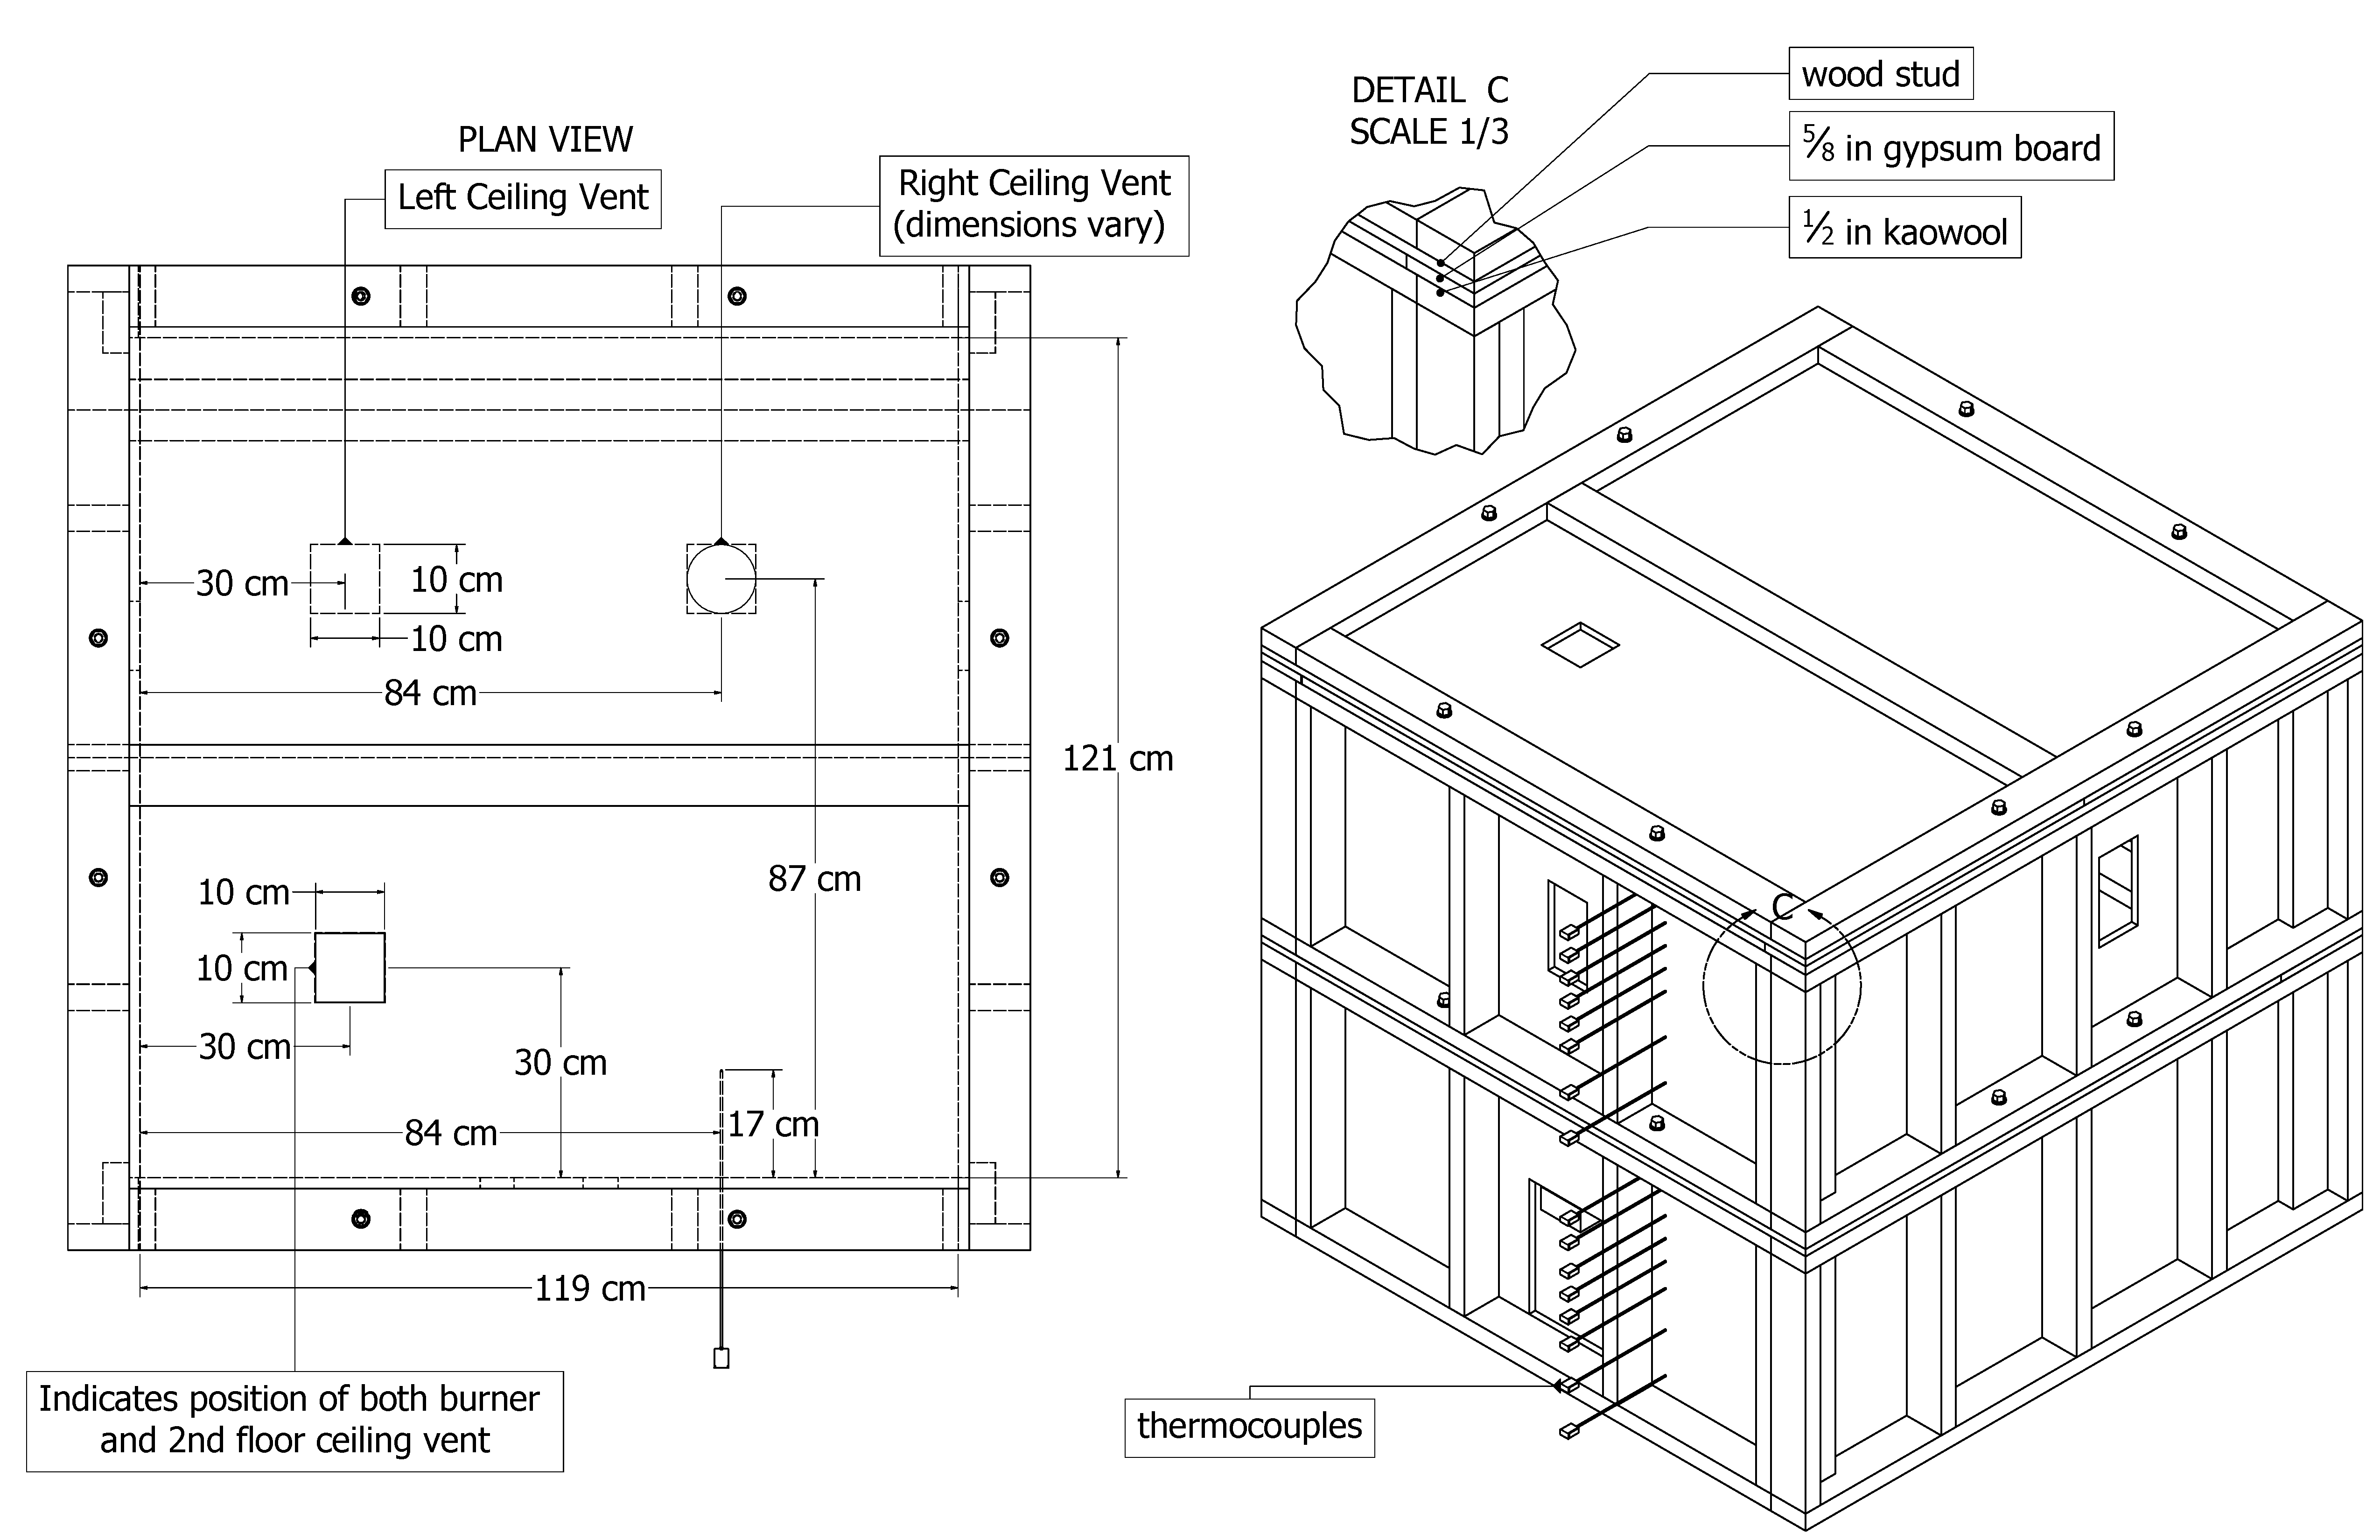
\includegraphics[width=\textwidth]{FIGURES/NIST_Vent_Study/Latex_Drawing_Plan}
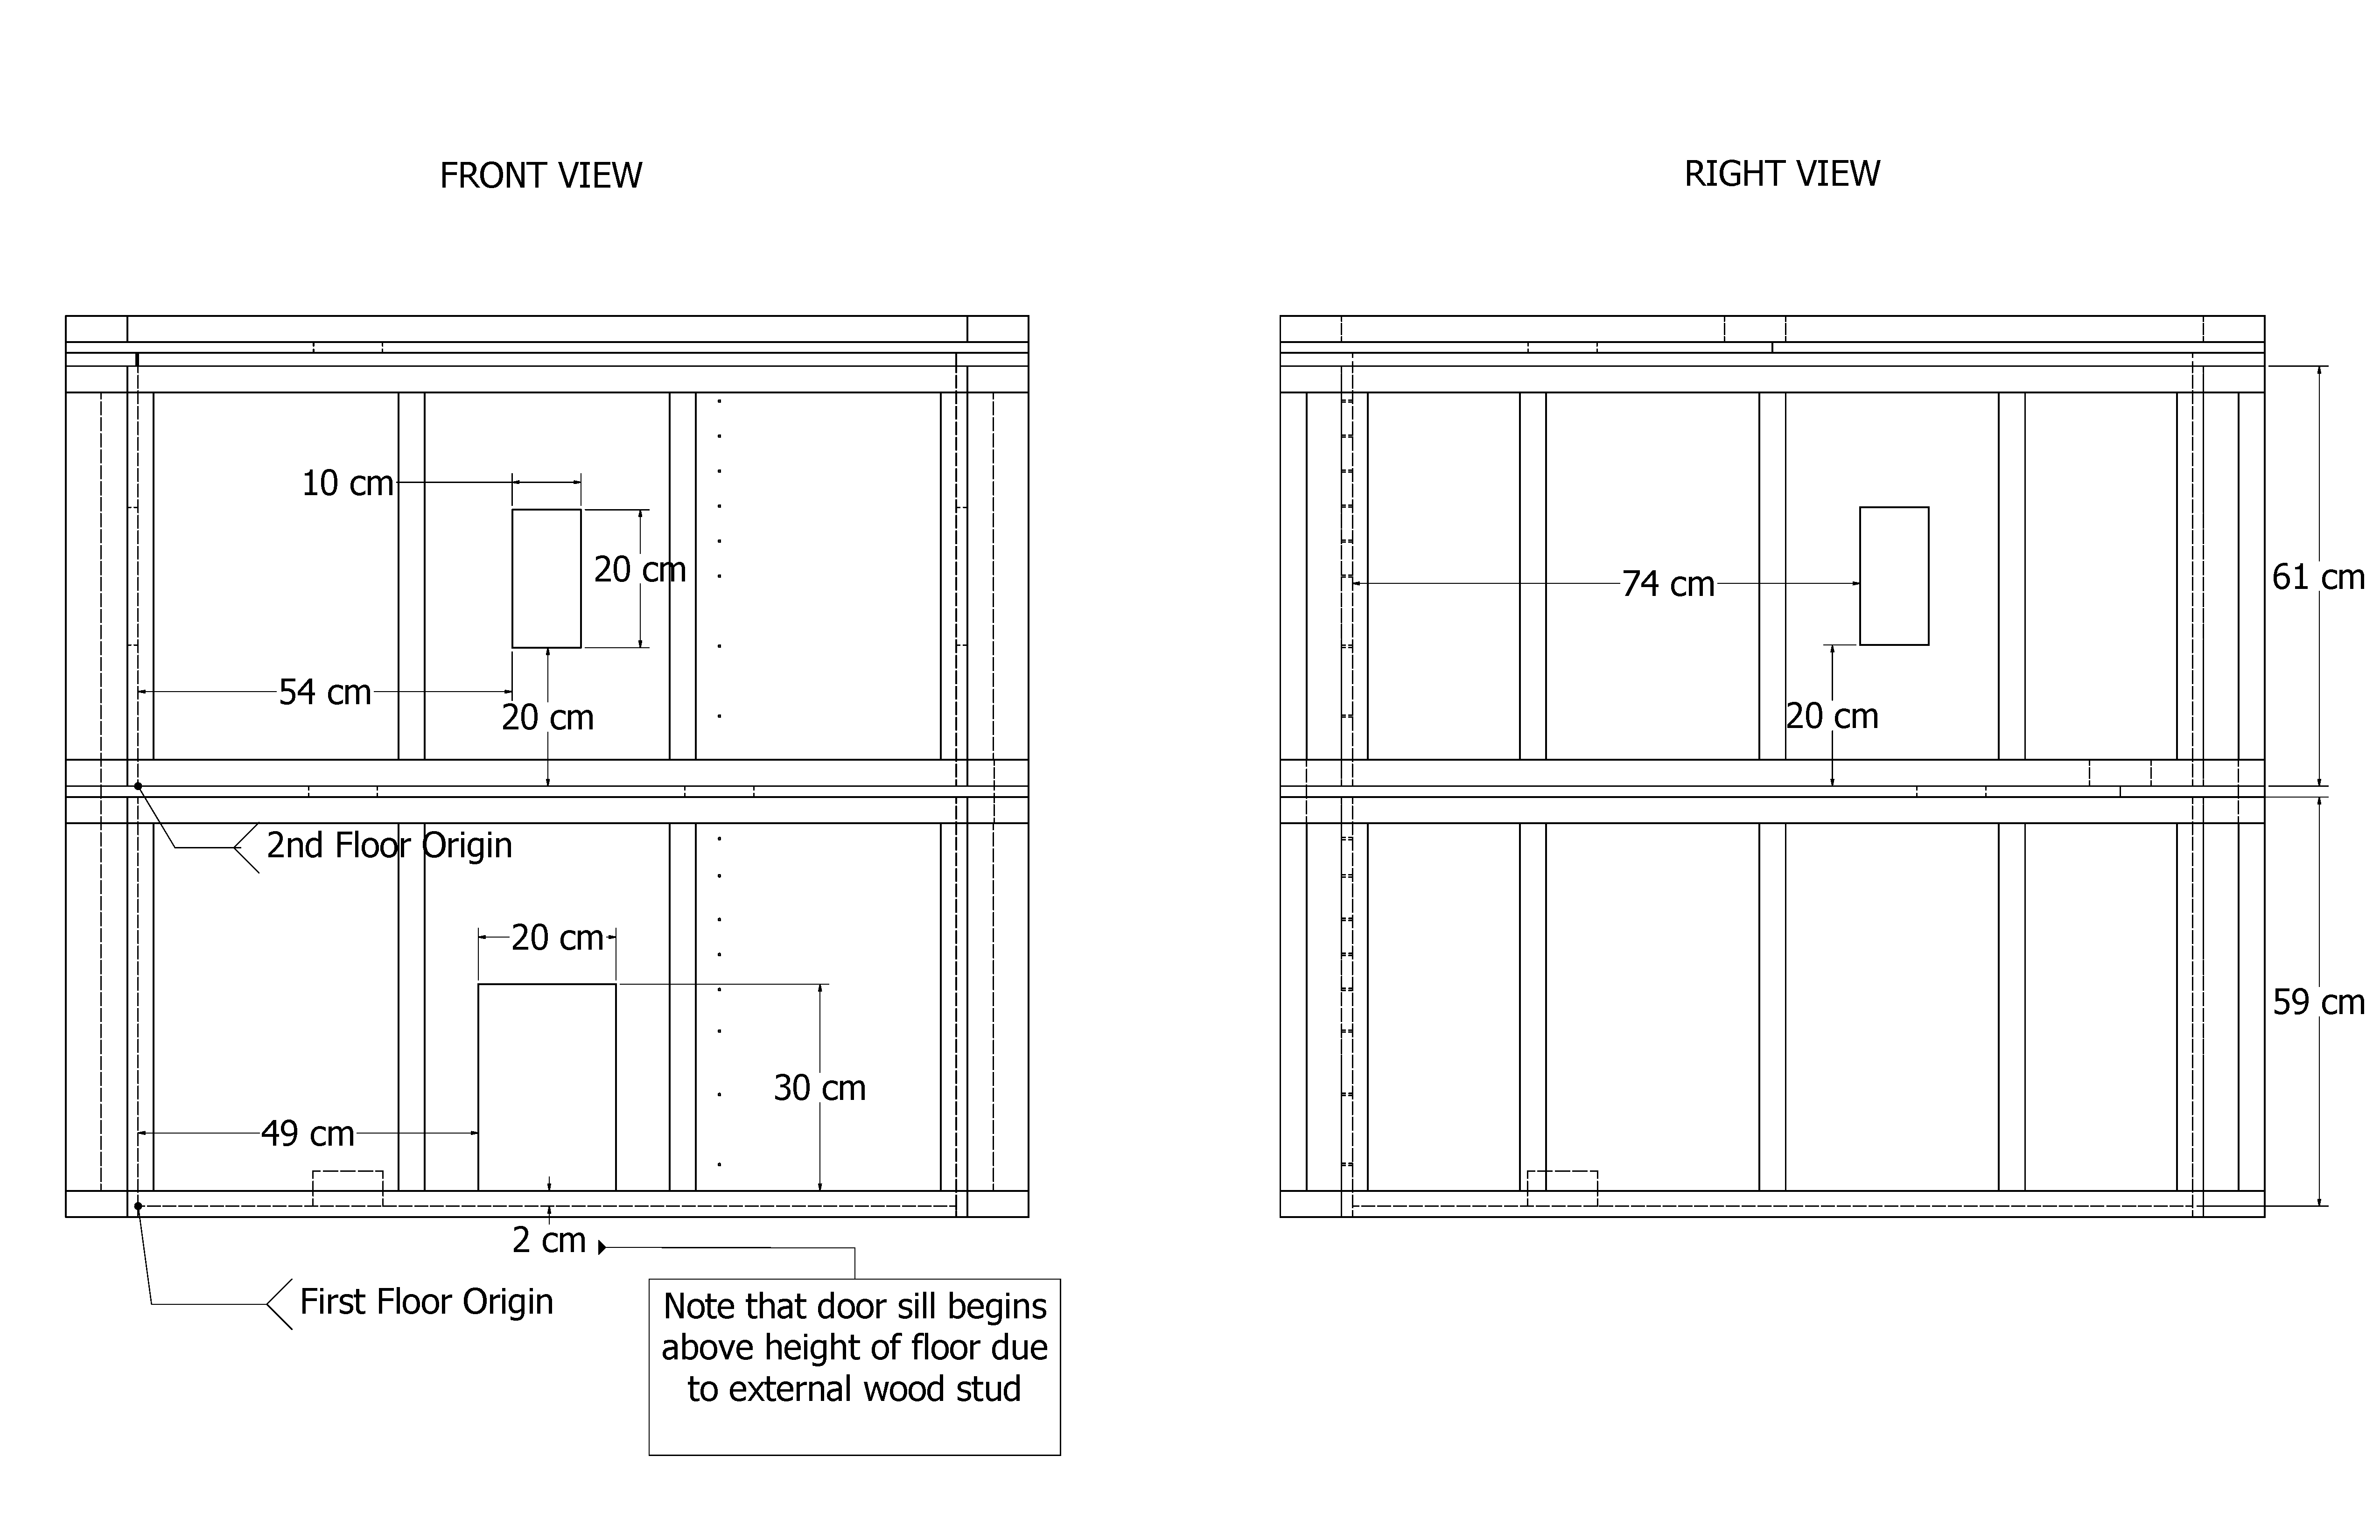
\includegraphics[width=\textwidth]{FIGURES/NIST_Vent_Study/Latex_Drawing_Front}
\caption[Geometry of the compartment from the NIST Vent Study]{Geometry of the compartment from the NIST Vent Study}
\label{NIST_Vent_Study_Drawing}
\end{figure}

\subsubsection{Material Properties}

The walls, ceiling and floor of each compartment was 1.6~cm (5/8~in) Type~X gypsum board. Wood studs formed the exterior frame. Thermo-physical properties of the gypsum board were taken from in Ref.~\cite{Manzello:SiF08} and manufacturer literature. It was assumed that the specific heat was 1.089~kJ/(kg $\cdot$ K), thermal conductivity 0.15~W/m/K, and density 673~kg/m$^3$.  Additionally, a  layer of kaowool, shown in Fig.~\ref{NIST_Vent_Study_Drawing} was used to seal the gap between the removable roof and the second story walls. Aluminum tape was used to seal all other seams.

\subsubsection{Burner}

For all experiments, a 10~cm square propane burner fueled at a rate of 1.65~L/min generated a 2.5~kW fire according to the following calculation:
\be
   1.65 \frac{\rm L}{\rm min} \times \frac{1}{60} \frac{\rm min}{\rm s} \times \frac{1}{1000} \frac{{\rm m}^3}{\rm L} \times 1.967 \, \frac{\rm kg}{{\rm m}^3} \times 46,300 \, \frac{\rm kJ}{\rm kg} = 2.50 \; {\rm kW}
\label{Conversion_Equation}
\ee
Note that the mass flow controller (Sierra Instruments SmartTrak~50) assumed standard conditions to be 0~$^\circ$C and 101325~Pa. For Tests~13-15, a Dwyer flow meter was used in place of the mass flow controller. The flow meter had a flow range of 4~L/min air.

\subsubsection{Thermocouples}

Eight Type-K thermocouples were inserted at each level to measure the vertical temperature profile. The thermocouples formed a vertical array at 84~cm from the left wall of the enclosure, and 17~cm from the front wall. TC-1 was defined as the uppermost thermocouple, with heights defined as the vertical distance from the compartment specific floor.

\begin{table}[h!]
\caption{Heights of the thermocouples above the floor of each level of the enclosure}
\begin{center}
\begin{tabular}{|c|c|c|c|c|c|c|c|c|c|c|c|c|c|c|c|c|}
\hline
Floor 2 TC's   & 1& 2& 3 & 4& 5& 6& 7&8\\ \hline
Height (cm) & 56.5& 50.8& 45.5& 41.0& 36.0& 29.8& 19.8& 10.5\\ \hline
Floor 1 TC's & 9&10&11&12&13&14&15&16\\ \hline
Height (cm) &51.8&47.0&40.64&35.6&30.48&25.7& 16.5&7.0\\ \hline


\end{tabular}
\end{center}
\label{Tab.TC}
\end{table}

\subsubsection{Test Procedure}

Each experiment lasted 100~min with a 5~min cool down period. Table~\ref{tab:NIST_Vent_Study} indicates the times when vents and windows were opened after the start of each experiment. For Test No. 1-4, two trials were performed. In each case, the difference in temperature remained within 3 percent, a difference of less than 1~$^\circ$C. For this reason, no further replicates were conducted.

\begin{table}[h!]
\caption{Vent State by Experiment: Time Opened}
\begin{center}
\begin{tabular}{|c|c|c|c|c|c|c|c|c|c|}
\hline
Test & Front    & Left    & Right     & Left     & Right   & Left         & Right        & Right   & Roof    \\
No.  & Window   & Window  & Window    & Vent     & Vent    & Vent Area    & Vent Area    & Vent    & Vent    \\
     & (min)    & (min)   & (min)     & (min)    & (min)   & (cm$^2$)     & (cm$^2$)     & Shape   & (min)   \\ \hline \hline
1    & 0        &  0      &  0        &  Closed  &  0      &  0           &  100         &  Square & Closed  \\ \hline
2    & 0        &  0      &  0        &  Closed  &  20     &  0           &  100         &  Square & Closed  \\ \hline
3    & 60       &  40     &  Closed   &  Closed  &  20     &  0           &  100         &  Square & Closed  \\ \hline
4    & 0        &  0      &  0        &  Closed  &  0      &  0           & 400          &  Square & Closed  \\ \hline
5    & 0        &  0      &  0        &  Closed  &  20     &  0           &  400         &  Square & Closed  \\ \hline
6    & 60       &  40     &  Closed   &  Closed  &  20     &  0           &  400         &  Square & Closed  \\ \hline
7    &  0       &  0      &  0        &  0       &  0      &  100         &  400         &  Square & Closed  \\ \hline
8    &  0       &  0      &  0        &  20      &  40     &  100         &  400         &  Square & Closed  \\ \hline
9    &  80      &  60     &  Closed   &  20      &  40     &  100         &  400         &  Square & Closed  \\ \hline
10   &  0       &  0      &  0        &  Closed  &  0      &  0           &  100         & Circle  & Closed  \\ \hline
11   &  0       &  0      &  0        &  Closed  &  20     &  0           &  100         & Circle  & Closed  \\ \hline
12   &  60      &  40     &  Closed   &  Closed  &  20     &  0           &  100         & Circle  & Closed  \\ \hline
13   &  0       &  0      &  0        &  0       &  0      &  100         &  400         &  Square & 0       \\ \hline
14   &  0       &  0      &  0        &  20      &  40     &  100         &  400         &  Square & 60      \\ \hline
15   &  Closed  & Closed  &  Closed   &  20      &  40     &  100         &  400         &  Square & 60      \\ \hline
\end{tabular}
\end{center}
\label{tab:NIST_Vent_Study}
\end{table}


\clearpage

\section{NRCC Facade Heat Flux Measurements}

A series of experiments was conducted by the Fire Research Section of the Institute for Research in Construction, National Research Council of Canada (NRCC), to measure the heat flux to a mock exterior building facade due to a fire within a compartment~\cite{Oleszkiewicz:ASME,Oleszkiewicz:FireTech}. The experiments selected for model validation were conducted using a series of propane line burners within a compartment whose interior dimensions were 5.95~m wide, 4.4~m deep, and 2.75~m high (see Fig.~\ref{NRCC_Facade_Drawing}). There were five different door/window sizes:
\begin{enumerate}
\item 0.94 m by 2.00 m high
\item 0.94 m by 2.70 m high (door)
\item 2.60 m by 1.37 m high (shown in Fig.~\ref{NRCC_Facade_Drawing})
\item 2.60 m by 2.00 m high
\item 2.60 m by 2.70 m high (door)
\end{enumerate}
There were four fire sizes: 5.5~MW, 6.9~MW, 8.6~MW, and 10.3~MW. In all, 19 experiments were conducted, with the exception of the 10.3~MW fire with Window~1. In each experiment, heat flux measurements were made 0.5~m, 1.5~m, 2.5~m, and 3.5~m above the top of the door/window.

\begin{figure}[p]
\includegraphics[width=\textwidth]{FIGURES/NRCC_Facade/NRCC_Facade}
\caption[Geometry of the NRCC Facade Experiments]{Geometry of the NRCC Facade Experiments.}
\label{NRCC_Facade_Drawing}
\end{figure}


\section{NRCC Smoke Tower Experiments}

In 2006 and 2007, the National Research Council of Canada (NRCC) conducted 10 fire experiments in a 10 story experimental facility in Almonte, Ontario to study smoke movement through the stair shaft to the upper floors of the building. Four of these experiments utilized actual commodities as fuel, and six utilized a propane burner. Four of the six propane fires were intended to reproduce the heat release of the commodity fires, and these experiments (BK-R, CMP-R, CLC-I-R, and CLC-II-R) have been chosen for this guide. Details of the experiments are included in a master's thesis and paper by Yan Wang~\cite{Wang:Thesis,Wang:FT2011}. A description of FDS simulations of the propane experiments not included in this guide is given by Hadjisophocleous and Jia~\cite{Hadjisophocleous:FT2009}. The analysis of the propane burner experiments discussed in this guide are based on the work of Paul Tyson at Ulster University as part of his master's thesis~\cite{Tyson:Thesis}.

\begin{figure}[p]
\includegraphics[width=\textwidth]{FIGURES/NRCC_Smoke_Tower/NRCC_Smoke_Tower}
\caption[Geometry of the NRCC Smoke Tower Experiments]{Geometry of the NRCC Smoke Tower Experiments.}
\label{NRCC_Smoke_Tower_Drawing}
\end{figure}

The tower was designed as a test bed for the center core of a high-rise building. It includes a compartment and corridor on each floor, a stair shaft, elevator shaft and service shafts~\cite{Achakji:1987}. Figure~\ref{NRCC_Smoke_Tower_Drawing} displays the geometry of the building as modeled in FDS. All walls and floor slabs are taken to be 0.2~m thick. The first two floors are 3.4~m high, slab to slab. The upper eight floors are 2.4~m, slab to slab. The propane burner was located on the second floor and the smoke flowed through open doors to the stair vestibule and stair shaft itself. In the four experiments considered in this guide, the stair shaft was open on the fourth, sixth, eighth, and tenth floors. The other floors were closed off to the stair shaft. The ventilation system was turned off. A single door was opened on the first floor, and there were no other openings to the outside save natural building leakage. The referenced documents do not explicitly include estimates of leakage areas, but for the sake of modeling, the leakage for each floor was concentrated at a single 1.5~m by 1.5~m exterior window. The leakage area was specified based on an estimate of a ``loose'' building exterior in NFPA~92~\cite{NFPA_92}. This is a very important consideration in modeling because it determines the extent to which the smoke rising up the stair shaft encounters an opposing downward flow.

Thermocouples and gas analyzers were placed at various locations to measure temperature and O$_2$, CO$_2$ and CO concentrations. A vertical array of TCs was located in the fire compartment and the doorway leading into the stair shaft on the second floor. TCs were also placed at each floor in the stair shaft. The gas analyzers were located in the stair shaft at the second floor, just outside the door to the fire compartment.



%\section{NRL Confined Space Experiments}
%
%The U.S. Naval Research Laboratory (NRL) performed a multi-year series of experiments inside of a four level,
%23 compartment test facility with 20 doors and ceiling vents whose exterior boundaries were airtight~\cite{Confined_JFPE} ~\cite{Confined_DTIC}.
%Three HVAC systems were installed in the facility: a supply air system that takes suction from a fan room and discharges the air to the each of the compartments,
%an exhaust system that takes suction from each of the compartments and discharges it to the fan room, and a smoke control control system that takes suction from an upper
%level compartment and discharges it to the ambient (see Figure~\ref{confined_HVAC}).
%A second set of HVAC ducts directly connected the second level with the fourth level (see Figure~\ref{confined_bypass}).
%
%\begin{figure}[ht]
%\begin{center}
%%\includegraphics[width=5.in]{FIGURES/NRL_Confined_Space/confined_space_hvac_layout}
%\end{center}
%\caption{Confined space HVAC system layouts.}
%\label{confined_HVAC}
%\end{figure}
%
%\begin{figure}[ht]
%\begin{center}
%%\includegraphics[width=5.in]{FIGURES/NRL_Confined_Space/confined_space_bypass}
%\end{center}
%\caption{Confined space bypass ducts.}
%\label{confined_bypass}
%\end{figure}
%
%The test facility was instrumented with gas thermocouples, surface thermocouples, optical density meters, gas sampling lines (CO$_2$, CO, and O$_2$),
%and velocity probes in a small number of doors, vents, and HVAC ducts.  Test variables included the number of opened doors and hatches, the number of vent openings to the ambient,
%the fire location, the fire size, and the operation of the HVAC systems.  All the fires were marine diesel pool fires.
%
%\clearpage


\section{NRL/HAI Wall Heat Flux Measurements}

Back, Beyler, DiNenno and Tatem~\cite{Back:IAFSS4} measured the heat flux from 9 different sized propane fires set up against a wall composed
of gypsum board. The experiments were sponsored by the Naval Research Laboratory and conducted by Hughes Associates, Inc., of Baltimore, Maryland. The
square sand burner ranged in size from 0.28~m to 0.70~m, and the fires ranged in size from 50~kW to 520~kW.

\section{PRISME Project}

PRISME is the name of a fire test program conducted under the auspices of the Organization for Economic Cooperation and Development, Nuclear Energy Agency (OECD/NEA). The experiments were conducted at the French Institut de radioprotection et de s\^{u}ret\'{e} nucl\'{e}aire (IRSN) at Cadarache. A variety of experiments were conducted to study ventilation effects, electrical cable failure, and leakage. The test reports are not publicly available, but an entire edition of {\em Fire Safety Journal} documented various experimental and modeling studies~\cite{Audouin:FSJ}.

The PRISME DOOR series consisted of six experiments, five of which involving two compartments connected by an open door (Tests 1-5) and one involving a third compartment (Test 6). The compartments were 5~m by 6~m by 4~m high. A well-instrumented ventilation system supplied air and exhausted combustion products at specified rates, but the thermal expansion of the gases caused these rates to change, a phenomenon that was intended to test the ventilation capabilities of the models. Wahlqvist and van Hees~\cite{Wahlqvist:FSJ} modeled these experiments using FDS and contributed the input files for the cases documented in this guide.

The PRISME LEAK series consisted of experiments where smoke and heat flowed through various types of leaks between the test compartments. Instrumented cables were placed at various locations, and gas and solid phase temperatures were measured. FDS was used to simulate the heating up of the cables using the measured gas temperature several centimeters from the cables~\cite{Dreisbach:Interflam}.

\section{Purdue Flames}

A turbulent buoyant diffusion flame is established on a diffuser burner with an exit diameter of 7.1 cm. The diverging angle of the burner is 7$^\circ$ such that the gaseous fuel (methane) is decelerated and forms a uniform velocity distribution at the burner exit \cite{Xin:CF2005}. The methane (CH4) mass flow rate (84.3 mg/s) The buoyant diffusion flame burns in a quiescent atmospheric pressure environment. The flame is surrounded by a screened enclosure to minimize flame disturbance. The Froude number of the flame is 0.109 and matches that of a 7.1 cm diameter liquid toluene pool fire \cite{Xin:CF2005,Zhou:CS1998}. The total heat release rate of the methane flame is 4.2 kW under the assumption of complete combustion, and the visible flame height is approximately 36 cm \cite{Xin:CF2005}. Measured and computed vertical and horizontal velocity, mixture fraction, and temperature values for this flame have been reported by Xin et al.~\cite{Xin:CF2005,Xin:PhD2002} and Zhou et al.~\cite{Zhou:CS1998,Zhou:PurduePhD1999}. The mean temperatures have been inferred from the measured species concentrations \cite{Xin:CF2005} by assuming an adiabatic flame. The interdependencies between species concentrations, temperature and specific heat have been ignored for determining the mean temperature.

\section{Restivo Compartment Air Flow Experiment}

Velocity measurements for forced airflow within a 9~m by 3~m by 3~m high compartment (Fig.~\ref{Restivo_Drawing}) were made by Restivo~\cite{Restivo:1979}. These measurements have been widely used to validate CFD models designed for indoor air quality applications. It was also used to assess early versions of FDS~\cite{Emmerich:1,Emmerich:2,Musser:1}. In the experiment, air was forced into the compartment through a 16.8~cm vertical slot along the ceiling running the width of the compartment with a velocity of 0.455~m/s. A passive exhaust was located near the floor on the opposite wall, with conditions specified such that there was no buildup of pressure in the enclosure. The component of velocity in the lengthwise direction was measured in four arrays: two vertical arrays located 3~m and 6~m  from the inlet along the
centerline of the room, and two horizontal arrays located 8.4~cm above the floor and below the ceiling, respectively. These measurements were taken using hot-wire anemometers. While data on the specific instrumentation used are not readily available, hot-wire systems tend to have limitations at low velocities, with typical thresholds of approximately 0.1~m/s.

\begin{figure}[ht]
\includegraphics[width=\textwidth]{FIGURES/Restivo_Experiment/Restivo_Drawing}
\caption[Geometry of Restivo's compartment]{Geometry of Restivo's compartment.}
\label{Restivo_Drawing}
\end{figure}

\section{Sandia Plume Experiments}

The Fire Laboratory for Accreditation of Models by Experimentation (FLAME) facility \cite{OHern:2005,Blanchat:2001} at Sandia National Laboratories in Albuquerque, New Mexico, is designed specifically for validating models of buoyant fire plumes.  The plume source is 1 m in diameter surrounded by a 0.5 m steel `ground plane'. PIV/PLIF techniques are used to obtain instantaneous joint scalar and velocity fields.  O'Hern et al.~\cite{OHern:2005} studied a turbulent buoyant helium plume in the FLAME facility. Earlier work to model this experiment has been performed by DesJardin et al.~\cite{DesJardin:2004}. Tieszen et al.~\cite{Tieszen:2004,Tieszen:2002} studied methane and hydrogen pool fires.

\section{Sippola Aerosol Deposition Experiments}

Mark Sippola, a doctoral student at the University of California, Berkeley, measured aerosol deposition velocities for various sizes of monodisperse fluorescent particles and various air velocities in a duct \cite{Sippola:2002,Sippola:2010}. For the experiments considered here, the straight steel duct with smooth walls was square with dimensions of 15~cm by 15~cm. The particle diameters were 1~$\mu$m, 3~$\mu$m, 5~$\mu$m, 9~$\mu$m, and 16~$\mu$m. The air velocities in the duct were 2.2~m/s, 5.3~m/s, and 9.0~m/s. A total of twelve panels (20~cm by 10~cm) were cut from the duct section to measure the amount of particles deposited to the duct surfaces; four panels each from the duct ceiling, wall, and floor surfaces. Fluorescent measurement techniques and aerosol concentration measurements were used to calculate the deposition velocities of the particles to duct surfaces (ceiling, wall, and floor) at two straight duct sections where the turbulent flow profile was fully developed.

\section{Smyth Slot Burner Experiment}

Kermit Smyth et al.~conducted diffusion flame experiments at NIST using a methane/air Wolfhard-Parker slot burner. The experiments are described in detail in Refs.~\cite{Norton:1,Smyth:1}. The Wolfhard-Parker slot burner consists of an 8~mm wide central slot flowing fuel surrounded by two 16~mm wide slots flowing dry air with 1~mm separations between the slots.
The slots are 41~mm in length. Measurements were made of all major species and a number of minor species along with temperature and velocity. Experimental uncertainties have been reported as 5~\% for temperature  and 10~\% to 20~\%
for the major species.

\section{SP Adiabatic Surface Temperature Experiments}

In 2008, three compartment experiments were performed at SP Technical Research Institute of Sweden under the sponsorship of Brandforsk, the Swedish Fire Research Board~\cite{Wickstrom_AST}. The objective of the experiments was to demonstrate how plate thermometer measurements in the vicinity of a simple steel beam can be used to supply the boundary conditions for a multi-dimensional heat conduction calculation for the beam. The adiabatic surface temperature was derived from the plate temperatures.

The experiments were performed inside a standard compartment designed for corner fire testing (ISO 9705). The compartment is 3.6~m deep, 2.4~m wide and 2.4~m high and includes a door opening 0.8~m by 2.0~m (Fig.~\ref{Room_Drawing}). The room was constructed of 20~cm thick light weight concrete blocks with a density of 600~kg/m$^3$~$\pm$~100~kg/m$^3$. The heat source was a gas burner run at a constant power of 450~kW. The top of the burner, with a square opening 30~cm by 30~cm, was placed 65~cm above the floor, 2.5~cm from the walls. A single steel beam was suspended 20~cm below the ceiling along the centerline of the compartment. There were three measurement stations along the beam at lengths of 0.9~m (Position A), 1.8~m (Position B), and 2.7~m (Position C) from the far wall where the fire was either positioned in the corner (Tests 1 and 2), or the center (Test 3). The beam in Test 1 was a rectangular steel tube filled with an insulation material. The beam in Tests 2 and 3 was an I-beam. A diagram of the room used in Test~2 is displayed in Figure~\ref{Room_Drawing}.

\begin{figure}[ht]
\includegraphics[width=\textwidth]{FIGURES/SP_AST/SP_AST_Compartment_Drawing}
\caption{Geometry of the  SP/AST compartment for Test 2.}
\label{Room_Drawing}
\end{figure}

A second series of experiments involving plate thermometers was carried out in 2011~\cite{Sjostrom:AST}. A 6~m long, 20~cm diameter vertical steel column was positioned in the center of 1.1~m and 1.9~m diesel fuel and 1.1~m heptane pool fires. Gas, plate thermometer, and surface temperatures were measured at heights of 1~m, 2~m, 3~m, 4~m, and 5~m above the pool surface. These experiments are notable because the column is partially engulfed in flames.

A third series of experiments involving plate thermometers was conducted in 2015~\cite{Sjostrom:SP2016}. A simple compartment with a single door was constructed and instrumented primarily with plate thermometers. The compartment was 2.7~m long, 1.8~m wide, and 1.8~m tall, with a 0.6~m by 1.5~m door centered on one of the short walls. The PTs were affixed to the walls. The 12 experiments were conducted with four different wall linings. In Series~A, the compartment was lined with a 10~cm thick light concrete block. In Series~B, the compartment was lined with a 5~cm thick layer of insulation backed by a 3~mm thick plate of steel. In Series~C, the compartment was lined with an uninsulated 3~mm thick steel plate. In Series~D, the compartment was lined with a 3~mm thick steel plate backed by a 5~cm thick layer of insulation (the opposite of Series~B). The fires were fueled by a 0.3~m by 0.3~m propane burner located in the center of the room except for Test~A3, where it was centered on the back wall. For most of the experiments, the heat release rate was 1000~kW, except for A2 and C1, which were 500~kW, and A4 and C3, which employed linear ramp-ups to 1250~kW.


\section{Steckler Compartment Experiments}

Steckler, Quintiere and Rinkinen performed a set of 55 compartment fire tests at NBS in 1979. The compartment was 2.8~m by 2.8~m by 2.13~m high\footnote{The test report gives the height of the compartment as 2.18~m. This is a misprint. The compartment was 2.13~m high.}, with a single door of various widths, or alternatively a single window with various heights. A 30~cm diameter methane burner was used to generate fires with heat release rates of 31.6~kW, 62.9~kW, 105.3~kW and 158~kW. Vertical profiles of velocity and temperature were measured in the doorway, along with a single vertical profile of temperature within the compartment. A full description and results are reported in Reference~\cite{Steckler:NBSIR_82-2520}. The basic test matrix is listed in Table~\ref{Steckler_Table}. Note that the test report does not include a detailed description of the compartment. However, an internal report\footnote{ {\em Technical Research Report, Fire Induced Flows Through Room Openings - Flow Coefficients}, Project 203005-003, Armstrong Cork Company, Lancaster, Pennsylvania, May, 1981.} by the test sponsor, Armstrong Cork Company, reports that the compartment floor was composed of 19~mm calcium silicate board on top of 12.7~mm plywood on wood joists. The walls and ceiling consisted of 12.7~mm ceramic fiber insulation board over 0.66~mm aluminum sheet attached to wood studs. A diagram of the compartment is displayed in Fig.~\ref{Steckler_ Drawing}.

\begin{table}[h!]
\caption{Summary of Steckler compartment experiments.}
\begin{center}
\begin{tabular}{|c|c|c|c|c||c|c|c|c|c|}
\hline
        & Door      & Door          &  HRR       & Burner       &       & Door      & Door        &  HRR         & Burner        \\
Test    & Width     & Height        & $\dot{Q}$  & Location     & Test  & Width     & Height      & $\dot{Q}$    & Location      \\
        & (m)       & (m)           & (kW)       &              &       & (m)       &  (m)        & (kW)         &                \\ \hline \hline
10      & 0.24      & 1.83          &  62.9      & Center       & 224   & 0.74      & 0.92        &  62.9         & Back Corner         \\ \hline
11      & 0.36      & 1.83          &  62.9      & Center       & 324   & 0.74      & 0.92        &  62.9         & Back Corner         \\ \hline
12      & 0.49      & 1.83          &  62.9      & Center       & 220   & 0.74      & 1.83        &  31.6         & Back Corner         \\ \hline
612     & 0.49      & 1.83          &  62.9      & Center       & 221   & 0.74      & 1.83        &  105.3        & Back Corner         \\ \hline
13      & 0.62      & 1.83          &  62.9      & Center       & 514   & 0.24      & 1.83        &  62.9         & Back Wall           \\ \hline
14      & 0.74      & 1.83          &  62.9      & Center       & 544   & 0.36      & 1.83        &  62.9         & Back Wall           \\ \hline
18      & 0.74      & 1.83          &  62.9      & Center       & 512   & 0.49      & 1.83        &  62.9         & Back Wall           \\ \hline
710     & 0.74      & 1.83          &  62.9      & Center       & 542   & 0.62      & 1.83        &  62.9         & Back Wall           \\ \hline
810     & 0.74      & 1.83          &  62.9      & Center       & 610   & 0.74      & 1.83        &  62.9         & Back Wall           \\ \hline
16      & 0.86      & 1.83          &  62.9      & Center       & 510   & 0.74      & 1.83        &  62.9         & Back Wall           \\ \hline
17      & 0.99      & 1.83          &  62.9      & Center       & 540   & 0.86      & 1.83        &  62.9         & Back Wall           \\ \hline
22      & 0.74      & 1.38          &  62.9      & Center       & 517   & 0.99      & 1.83        &  62.9         & Back Wall           \\ \hline
23      & 0.74      & 0.92          &  62.9      & Center       & 622   & 0.74      & 1.38        &  62.9         & Back Wall           \\ \hline
30      & 0.74      & 0.92          &  62.9      & Center       & 522   & 0.74      & 1.38        &  62.9         & Back Wall           \\ \hline
41      & 0.74      & 0.46          &  62.9      & Center       & 524   & 0.74      & 0.92        &  62.9         & Back Wall           \\ \hline
19      & 0.74      & 1.83          &  31.6      & Center       & 541   & 0.74      & 0.46        &  62.9         & Back Wall           \\ \hline
20      & 0.74      & 1.83          &  105.3     & Center       & 520   & 0.74      & 1.83        &  31.6         & Back Wall           \\ \hline
21      & 0.74      & 1.83          &  158.0     & Center       & 521   & 0.74      & 1.83        &  105.3        & Back Wall           \\ \hline
114     & 0.24      & 1.83          &  62.9      & Back Corner  & 513   & 0.74      & 1.83        &  158.0        & Back Wall           \\ \hline
144     & 0.36      & 1.83          &  62.9      & Back Corner  & 160   & 0.74      & 1.83        &  62.9         & Center$^*$          \\ \hline
212     & 0.49      & 1.83          &  62.9      & Back Corner  & 163   & 0.74      & 1.83        &  62.9         & Back Corner$^*$     \\ \hline
242     & 0.62      & 1.83          &  62.9      & Back Corner  & 164   & 0.74      & 1.83        &  62.9         & Back Wall$^*$       \\ \hline
410     & 0.74      & 1.83          &  62.9      & Back Corner  & 165   & 0.74      & 1.83        &  62.9         & Left Wall$^*$       \\ \hline
210     & 0.74      & 1.83          &  62.9      & Back Corner  & 162   & 0.74      & 1.83        &  62.9         & Right Wall$^*$      \\ \hline
310     & 0.74      & 1.83          &  62.9      & Back Corner  & 167   & 0.74      & 1.83        &  62.9         & Front Center$^*$    \\ \hline
240     & 0.86      & 1.83          &  62.9      & Back Corner  & 161   & 0.74      & 1.83        &  62.9         & Doorway$^*$         \\ \hline
116     & 0.99      & 1.83          &  62.9      & Back Corner  & 166   & 0.74      & 1.83        &  62.9         & Front Corner$^*$    \\ \hline
122     & 0.74      & 1.38          &  62.9      & Back Corner  &  \multicolumn{5}{r|}{$^*$ Raised burner}                   \\ \hline
\end{tabular}
\end{center}
\label{Steckler_Table}
\end{table}


\begin{figure}[p]
\includegraphics[width=\textwidth]{FIGURES/Steckler_Compartment/Steckler_Room_Drawing}
\caption{Geometry of the Steckler Compartment Experiments.}
\label{Steckler_ Drawing}
\end{figure}




\section{UL/NIST Vent Experiments}
\label{UL_NIST_Vents_Description}

In 2012, the Fire Fighting Technology Group at NIST conducted experiments at Underwriters Laboratories (UL) in Northbrook, Illinois, to assess the change in compartment temperature due to the opening of one or two 1.2~m square ceiling vents~\cite{Opert:Masters}. Four experiments were conducted using a natural gas burner in a 6.1~m by 4.3~m by 2.4~m compartment with a single door opening. The fires ranged in size from 500~kW to 2~MW, and the vents were opened and closed such that during the four experiments there were 31 discrete time intervals in which model predictions could be compared to quasi-steady conditions. The compartment contained two vertical arrays of thermocouples, and the door and vents were instrumented with thermocouples and bi-directional velocity probes. Only the thermocouple data has been used in the validation study. A diagram of the compartment is displayed in Figure~\ref{UL_NIST_Drawing}. The major test parameters are listed in Table~\ref{UL_NIST_Table}.

\begin{figure}[ht]
\includegraphics[width=\textwidth]{FIGURES/UL_NIST_Vents/UL_NIST_Vents_Drawing}
\caption{Geometry of the UL/NIST Experiments.}
\label{UL_NIST_Drawing}
\end{figure}


\begin{table}[h!]
\caption[Summary of UL/NIST Vent experiments]{Summary of UL/NIST Vent experiments. Note that the 31 ``experiments'' are actually discrete time intervals during the course of four separate fires.}
\begin{center}
\begin{tabular}{|c|c|c|c||c|c|c|c|}
\hline
Exp.    & End Time  & HRR           &  No. of   & Exp.    & End Time  & HRR           &  No. of           \\
No.     & (s)       & (kW)          & Vents     & No.     & (s)       & (kW)          & Vents             \\ \hline \hline
\multicolumn{4}{|c||}{Fire 1}                   & \multicolumn{4}{|c|}{Fire 3}                            \\ \hline
1       & 1215      & 430           & 0         & 14      & 453       & 476           & 0                 \\ \hline
2       & 1840      & 430           & 1         & 15      & 816       & 476           & 1                 \\ \hline
3       & 2168      & 430           & 2         & 16      & 1153      & 476           & 2                 \\ \hline
4       & 2474      & 430           & 0         & 17      & 1640      & 1002          & 0                 \\ \hline
5       & 2955      & 1011          & 0         & 18      & 1936      & 1002          & 1                 \\ \hline
6       & 3170      & 1011          & 1         & 19      & 2233      & 1002          & 2                 \\ \hline
7       & 3604      & 1011          & 2         & \multicolumn{4}{|c|}{Fire 4}                            \\ \hline
8       & 3840      & 1011          & 0         & 20      & 519       & 1011          & 0                 \\ \hline
9       & 4153      & 2188          & 0         & 21      & 967       & 1011          & 1                 \\ \hline
10      & 4284      & 2188          & 1         & 22      & 1325      & 1011          & 2                 \\ \hline
\multicolumn{4}{|c||}{Fire 2}                   & 23      & 1559      & 470           & 2                 \\ \hline
11      & 565       & 2144          & 0         & 24      & 1653      & 470           & 1                 \\ \hline
12      & 833       & 2144          & 1         & 25      & 2013      & 470           & 0                 \\ \hline
13      & 931       & 2144          & 2         & 26      & 2411      & 470           & 1                 \\ \hline
\multicolumn{4}{|r||}{}                         & 27      & 2910      & 470           & 2                 \\ \cline{5-8}
\multicolumn{4}{|r||}{}                         & 28      & 3399      & 2188          & 2                 \\ \cline{5-8}
\multicolumn{4}{|r||}{}                         & 29      & 3586      & 2188          & 0                 \\ \cline{5-8}
\multicolumn{4}{|r||}{}                         & 30      & 3803      & 2188          & 1                 \\ \cline{5-8}
\multicolumn{4}{|r||}{}                         & 31      & 4035      & 2188          & 2                 \\ \hline
\end{tabular}
\end{center}
\label{UL_NIST_Table}
\end{table}




\section{UL/NFPRF Sprinkler, Vent, and Draft Curtain Study}
\label{UL_NFPRF_Description}

In 1997, thirty-four heptane spray burner and five racked commodity experiments were conducted at the Large Scale Fire Test Facility at Underwriters Laboratories (UL) in Northbrook, Illinois~\cite{Sheppard:1,McGrattan:5}. The spray burner experiments were divided into two test series. Series I consisted of 22 4.4~MW experiments. Series~II consisted of 12 10~MW experiments. The objective of the spray burner experiments was to characterize the temperature and flow field for fire scenarios with a controlled heat release rate in the presence of sprinklers, draft curtains, and smoke \& heat vents.

The Large Scale Fire Test Facility at UL contains a 37~m by 37~m (120~ft by 120~ft) main fire test cell, equipped with a 30.5~m by 30.5~m (100~ft by 100~ft) adjustable height ceiling. The UL/NFPRF test results (Series I) are summarized in Table~\ref{ULmatrix}. The UL/NFPRF test results (Series II) are summarized in Table~\ref{ULburnermatrixII}. The layout of the experiments is shown in Figs.~\ref{layout}, \ref{burnerlayoutA}, and \ref{layout3}.

\begin{table}[h!]
\begin{center}
\begin{tabular}{|c||c|c|c|c|c|c|}
\hline
\multicolumn{7}{|c|}{\bf Heptane Spray Burner Test Series I}  \\ \hline \hline
Test & Burner & Vent                    & First         & Total      & Draft    & Heat Release Rate \\
No.  & Pos.   & Operation               & Actuation (s) & Actuations & Curtains & MW @ s \\
\hline \hline
I-1   & B  & Closed                     & 65            & 11        & Yes  & 4.4 @ 50  \\ \hline
I-2   & B  & Manual (0:40)              & 66            & 12        & Yes  & 4.4 @ 50  \\ \hline
I-3   & B  & Manual (1:30)              & 64            & 12        & Yes  & 4.4 @ 50  \\ \hline
I-4   & C  & Closed                     & 60            & 10        & Yes  & 4.4 @ 50  \\ \hline
I-5   & C  & Manual (0:40)              & 72            & 9         & Yes  & 4.4 @ 50  \\ \hline
I-6   & C  & Manual (1:30)              & 62            & 8         & Yes  & 4.4 @ 50  \\ \hline
I-7   & C  & 74$^\circ$C link (DNO)     & 70            & 10        & Yes  & 4.4 @ 50  \\ \hline
I-8   & B  & 74$^\circ$C link (9:26)    & 60            & 11        & Yes  & 4.4 @ 50  \\ \hline
I-9   & D  & 74$^\circ$C link (DNO)     & 70            & 12        & Yes  & 4.4 @ 50  \\ \hline
I-10  & D  & Manual (0:40)              & 72            & 13        & Yes  & 4.4 @ 50  \\ \hline
I-11  & D  & 74$^\circ$C link (4:48)    & N/A           & N/A       & Yes  & 4.4 @ 50  \\ \hline
I-12  & A  & Closed                     & 68            & 14        & Yes  & 4.4 @ 50  \\ \hline
I-13  & A  & 74$^\circ$C link (1:04)    & 69            & 5         & Yes  & 6.0 @ 60  \\ \hline
I-14  & A  & Manual (0:40)              & 74            & 7         & Yes  & 5.8 @ 60  \\ \hline
I-15  & A  & Manual (1:30)              & 64            & 5         & Yes  & 5.8 @ 60  \\ \hline
I-16  & A  & 74$^\circ$C link (1:46)    & 106           & 4         & Yes  & 5.0 @ 110 \\ \hline \hline
I-17  & B  & 100$^\circ$C link (DNO)    & 58            & 4         & No   & 4.6 @ 50 \\ \hline
I-18  & C  & 100$^\circ$C link (DNO)    & 58            & 4         & No   & 3.7 @ 50 \\ \hline
I-19  & A  & 100$^\circ$C link (10:00)  & 56            & 10        & No   & 4.6 @ 50 \\ \hline
I-20  & A  & 74$^\circ$C link (1:20)    & 54            & 4         & No   & 4.2 @ 50 \\ \hline
I-21  & C  & 74$^\circ$C link (7:00)    & 58            & 10        & No   & 4.6 @ 50 \\ \hline
I-22  & D  & 100$^\circ$C link (DNO)    & 60            & 6         & No   & 4.6 @ 50 \\ \hline
\end{tabular}
\end{center}
\caption[Results of the UL/NFPRF heptane spray experiments, Series~I]
{Results of Series~I of the UL/NFPRF heptane spray experiments. Note that DNO means ``Did Not Open''. Also note, the fires grew at a rate proportional to the square of the time until a certain flow rate of fuel was achieved at which time the flow rate was held steady. Thus, the ``Heat Release Rate'' was the size of the fire at the time when the fuel supply was leveled off.}
\label{ULmatrix}
\end{table}

\begin{figure}[p]
\begin{center}
\setlength{\unitlength}{.05416667in}
\begin{picture}(120,120)

\linethickness{1.mm} \put(0,0){\framebox(120,120)[tc]{North Wall}} \linethickness{.5mm} \put(10,10){\framebox(100,100)[tc]{Adjustable Height
Ceiling}}

\thinlines \put(117,67){\vector(0,-1){67}} \put(117,73){\vector(0, 1){47}} \put(117,70){\makebox(0,0){$120'$}} \put(113,57){\vector(0,-1){47}}
\put(111,110){\line(1,0){4.}} \put(111, 10){\line(1,0){4.}} \put(113,63){\vector(0, 1){47}} \put(113,60){\makebox(0,0){$100'$}}
\put(30.9,12.83){\dashbox{1}(67.1,71.17)[tc]{Draft Curtains}} \put(27.9,40){\vector(0,-1){27.17}} \put(27.9,46){\vector(0, 1){38.0}}
\put(25.9,84.){\line(1,0){4.}} \put(25.9,12.83){\line(1,0){4.}} \put(27.9,43){\makebox(0,0){$71'2''$}} \put(64.0,87.){\vector(-1,0){33.1}}
\put(72.0,87.){\vector( 1,0){26.0}} \put(30.9,85.){\line(0,1){4.}} \put(98.0,85.){\line(0,1){4.}} \put(68.0,87.){\makebox(0,0){$67'1''$}}

\put(16.0,87.){\vector(-1,0){6.}} \put(24.0,87.){\vector( 1,0){6.92}} \put(20.0,87.){\makebox(0,0){$20'11''$}} \put(101.,87.){\vector(-1,0){3.}}
\put(107.,87.){\vector( 1,0){3.}} \put(104.,87.){\makebox(0,0){$12'$}}

\put(27.9,100){\vector(0,1){10.}} \put(27.9,94){\vector(0,-1){10.}} \put(27.9,97){\makebox(0,0){$26'$}}

\put(27.9,8){\vector(0,1){2.}} \put(27.9,8){\line(1,0){3.}} \put(30.9,8){\makebox(0,0)[l]{$2'10''$}}

\put(55.08,14.83){\line(-1,0){2.}} \put(54.08,16.83){\vector(0,-1){2.}} \put(54.08,7.83){\vector(0,1){5.}} \put(54.08,7.83){\line(1,0){3.}}
\put(57.08,7.83){\makebox(0,0)[l]{$2'$}}

\put(85.08,24.83){\line(0,-1){2.}} \put(95.08,24.83){\line(0,-1){2.}} \put(93.08,23.83){\vector(1,0){2.}} \put(87.08,23.83){\vector(-1,0){2.}}
\put(103.00,23.83){\vector(-1,0){5.}} \put(103.00,23.83){\line(0,-1){3.}} \put(103.00,20.83){\makebox(0,0)[ct]{$2'11''$}}
\put(90.08,23.83){\makebox(0,0)[c]{$10'$}}

\thicklines \put(78.08,55.83){\framebox(4,8){ }}

\put(78.58,58.33){\framebox(3,3)[c]{A}} \put(78.58,68.33){\framebox(3,3)[c]{B}} \put(88.58,58.33){\framebox(3,3)[c]{C}}
\put(58.58,38.33){\framebox(3,3)[c]{D}}

\thinlines

\multiput(35.08,14.83)(0,10){7}{\circle*{.8}} \multiput(45.08,14.83)(0,10){7}{\circle*{.8}} \multiput(55.08,14.83)(0,10){7}{\circle*{.8}}
\multiput(65.08,14.83)(0,10){7}{\circle*{.8}} \multiput(75.08,14.83)(0,10){7}{\circle*{.8}} \multiput(85.08,14.83)(0,10){7}{\circle*{.8}}
\multiput(95.08,14.83)(0,10){7}{\circle*{.8}} \tiny \put(35.48,15.23){98} \put(45.48,15.23){91} \put(55.48,15.23){84} \put(65.48,15.23){81}
\put(75.48,15.23){78} \put(85.48,15.23){75} \put(95.48,15.23){72} \put(35.48,25.23){99} \put(45.48,25.23){92} \put(55.48,25.23){85}
\put(65.48,25.23){82} \put(75.48,25.23){79} \put(85.48,25.23){76} \put(95.48,25.23){73} \put(35.48,35.23){100} \put(45.48,35.23){93}
\put(55.48,35.23){86} \put(65.48,35.23){83} \put(75.48,35.23){80} \put(85.48,35.23){77} \put(95.48,35.23){74} \put(35.48,45.23){101}
\put(45.48,45.23){94} \put(55.48,45.23){87} \put(65.48,45.23){62} \put(75.48,45.23){58} \put(85.48,45.23){54} \put(95.48,45.23){50}
\put(35.48,55.23){102} \put(45.48,55.23){95} \put(55.48,55.23){88} \put(65.48,55.23){63} \put(75.48,55.23){59} \put(85.48,55.23){55}
\put(95.48,55.23){51} \put(35.48,65.23){103} \put(45.48,65.23){96} \put(55.48,65.23){89} \put(65.48,65.23){64} \put(75.48,65.23){60}
\put(85.48,65.23){56} \put(95.48,65.23){52} \put(35.48,75.23){104} \put(45.48,75.23){97} \put(55.48,75.23){90} \put(65.48,75.23){65}
\put(75.48,75.23){61} \put(85.48,75.23){57} \put(95.48,75.23){53} \put(70.08,49.83){\makebox(0,0)[c]{68}} \put(70.08,59.83){\makebox(0,0)[c]{69}}
\put(70.08,69.83){\makebox(0,0)[c]{70}} \put(80.08,49.83){\makebox(0,0)[c]{67}} \put(90.08,49.83){\makebox(0,0)[c]{66}}
\put(90.08,69.83){\makebox(0,0)[c]{71}}

\multiput(80.08,56.83)(0,1){7}{\circle*{.2}} \put(80.58,62.83){\line(1,0){22.5}} \put(104.,62.83){\makebox(0,0)[l]{43}}
\put(104.,61.33){\makebox(0,0)[l]{44}} \put(104.,59.83){\makebox(0,0)[l]{45}} \put(104.,58.33){\makebox(0,0)[l]{46}}
\put(104.,56.83){\makebox(0,0)[l]{47}} \put(104.,55.33){\makebox(0,0)[l]{48}} \put(104.,53.83){\makebox(0,0)[l]{49}}

\normalsize

\end{picture}
\end{center}
\caption[Plan view of the UL/NFPRF heptane spray experiments, Series~I.] {Plan view of the UL/NFPRF heptane spray experiments, Series~I. The sprinklers are indicated by the solid circles and are spaced exactly 10~ft apart. The number beside each sprinkler location indicates the channel number of the nearest thermocouple. The vent dimensions are 4~ft by 8~ft. The boxed letters A, B, C and D indicate burner positions. Corresponding to each burner position is a vertical array of thermocouples. Thermocouples 1--9 hang 7, 22, 36, 50, 64, 78, 92, 106 and 120~in from the ceiling, respectively, above Position A. Thermocouples 10 and 11 are positioned above and below the ceiling tile directly above Position B, followed by 12--20 that hang at the same levels below the ceiling as 1--9. The same pattern is followed at Positions C and D, with thermocouples 21--31 at C and 32--42 at D.}
\label{layout}
\end{figure}




\begin{table}[ht!]
\begin{center}
\begin{tabular}{|c||c|c|c|c|c|c|c|}
\hline
\multicolumn{8}{|c|}{\bf Heptane Spray Burner Test Series II (10 MW Fires)}\\ \hline \hline
Test & Burner   & Vent      & Sprinklers & First      & Last      & \multicolumn{2}{|c|}{Avg.~Peak Temp.} \\ \cline{7-8}
No.  & Position & Operation & Opened     & Activation & Activation & $^\circ$C & $^\circ$F   \\
\hline \hline
II-1  & D  & 74$^\circ$C link (DNO)  & 27 & 1:15 & 6:13 & 129.4 &264.9 \\ \hline
II-2  & D  & All Open at Start       & 28 & 1:05 & 5:53 & 128.8 &263.8 \\ \hline
II-3  & A  & 74$^\circ$C link (1:15) & 12 & 1:08 & 4:00 & 101.8 &215.2 \\ \hline
II-4  & B  & 74$^\circ$C link (1:48) & 16 & 1:03 & 5:54 & 108.8 &227.8 \\ \hline
II-5  & D  & 74$^\circ$C link (DNO)  & 28 & 1:10 & 7:07 & 130.0 &266.0 \\ \hline
II-6  & D  & All Open at Start       & 27 & 1:10 & 5:21 & 127.5 &261.5 \\ \hline
II-7  & A  & Closed                  & 18 & 1:09 & 4:11 & 117.2 &243.0 \\ \hline
II-8  & B  & 74$^\circ$C link (1:12) & 13 & 1:10 & 3:34 & 107.7 &225.9 \\ \hline
II-9  & E  & 74$^\circ$C link (DNO)  & 23 & 1:07 & 3:28 & 115.8 &240.4 \\ \hline
II-10 & F  & 74$^\circ$C link (3:20) & 19 & 1:14 & 3:01 & 108.4 &227.1 \\ \hline
II-11 & C  & 74$^\circ$C link (DNO)  & 23 & 1:02 & 3:56 & 123.4 &254.1 \\ \hline
II-12 & C  & All Open at Start       & 23 & 0:58 & 4:55 & 119.0 &246.2 \\ \hline
\end{tabular}
\end{center}
\caption[Results of the UL/NFPRF heptane spray experiments, Series~II]
{Results of the UL/NFPRF heptane spray experiments, Series II. Note that all fires were ramped up to 10~MW in 75~s following a $t$-squared curve.}
\label{ULburnermatrixII}
\end{table}


\begin{figure}[p]
\begin{center}
\setlength{\unitlength}{.054166in}
\begin{picture}(120,120)

\linethickness{1mm}
\put(0,0){\framebox(120,120)[tc]{ }}
\put(60,118){\makebox(0,0){North Wall}}
\put(60,  2){\makebox(0,0){South Wall}}

\linethickness{.5mm}
\put(10,10){\framebox(100,100)[tl]{ }}

\thinlines
\put(117,67){\vector(0,-1){67}}
\put(117,73){\vector(0, 1){47}}
\put(117,70){\makebox(0,0){$120'$}}
\put(113,57){\vector(0,-1){47}}
\put(113,63){\vector(0, 1){47}}
\put(113,60){\makebox(0,0){$100'$}}
\put(10.0,86.0){\dashbox{1}(30.0,24.0)[tl]{ }}
\put(40.,10.5){\dashbox{1}(69.5,75.5)[tl]{              }}

\thicklines
\put(48.,16.){\framebox(4,8){ }}
\put(48.,67.){\framebox(4,8){ }}
\put(28.,67.){\framebox(4,8){ }}
\put(98.,67.){\framebox(4,8){ }}
\put(98.,16.){\framebox(4,8){ }}

\large
\put(68.5,49.5){\dashbox{.5}(3,3)[c]{D}}
\put(48.5,69.5){\dashbox{.5}(3,3)[c]{A}}
\put(48.5,79.5){\dashbox{.5}(3,3)[c]{B}}
\put(58.5,59.5){\dashbox{.5}(3,3)[c]{C}}
\put(38.5,54.5){\dashbox{.5}(3,3)[c]{E}}
\put(38.5,84.5){\dashbox{.5}(3,3)[c]{F}}
\normalsize

\multiput(15,11)(0,10){10}{\circle*{.8}}
\multiput(25,11)(0,10){10}{\circle*{.8}}
\multiput(35,11)(0,10){10}{\circle*{.8}}
\multiput(45,11)(0,10){10}{\circle*{.8}}
\multiput(55,11)(0,10){10}{\circle*{.8}}
\multiput(65,11)(0,10){10}{\circle*{.8}}
\multiput(75,11)(0,10){10}{\circle*{.8}}
\multiput(85,11)(0,10){10}{\circle*{.8}}
\multiput(95,11)(0,10){10}{\circle*{.8}}
\multiput(105,11)(0,10){10}{\circle*{.8}}

\end{picture}
\end{center}
\caption[Plan view of the UL/NFPRF heptane spray experiments, Series~II ]
{Plan view of the UL/NFPRF heptane spray experiments, Series~II. The boxed letters A, B, C, D, E and F indicate burner positions. The sprinklers are indicated by the solid circles and are spaced exactly 10~ft apart. The vents are 4~ft by 8~ft. }
\label{burnerlayoutA}
\end{figure}

\setlength{\unitlength}{.054166in}
\newsavebox{\eightbox}
\savebox{\eightbox}(3.5,3.5){%
\put(0,0){\framebox(3.5,3.5){ }}
\put(1.75,0){\line(0,1){3.5}}
\put(0,1.75){\line(1,0){3.5}}}

\newsavebox{\onebox}
\savebox{\onebox}(3.5,3.5){%
\put(0,0){\framebox(3.5,3.5){ }}}

\thinlines
\newsavebox{\fuel}
\savebox{\fuel}(31.5,30.5){%
\multiput( 0.000, 0.0)(4.000,0){ 2}{\usebox{\onebox}}
\multiput( 8.000, 0.0)(4.000,0){ 4}{\usebox{\eightbox}}
\multiput(24.000, 0.0)(4.000,0){ 2}{\usebox{\onebox}}
\multiput( 0.000,11.5)(4.000,0){8}{\usebox{\eightbox}}
\multiput( 0.000,15.5)(4.000,0){8}{\usebox{\eightbox}}
\multiput( 0.000,27.0)(4.000,0){ 2}{\usebox{\onebox}}
\multiput( 8.000,27.0)(4.000,0){ 4}{\usebox{\eightbox}}
\multiput(24.000,27.0)(4.000,0){ 2}{\usebox{\onebox}}
\put(15.000,13.25){\framebox(.5,.5){ }}
\put(16.000,12.75){\framebox(.5,.5){ }}
\put(16.000,13.25){\framebox(.5,.5){ }}
\put(15.000,12.75){\framebox(.5,.5){ }}
}

\begin{figure}[p]
\begin{center}
\setlength{\unitlength}{.054166in}
\begin{picture}(120,120)

\linethickness{1mm}
\put(0,0){\framebox(120,120)[tc]{ }}
\put(60,118){\makebox(0,0){North Wall}}
\put(60,  2){\makebox(0,0){South Wall}}

\linethickness{.5mm}
\put(10,10){\framebox(100,100)[tl]{ }}

\thinlines
\put(10.0,86.0){\dashbox{1}(30.0,24.0)[tl]{ }}
\put(40.,10.5){\dashbox{1}(69.5,75.5)[tl]{              }}

\thicklines
\put(48.,16.){\framebox(4,8){ }}
\put(48.,67.){\framebox(4,8){ }}
\put(28.,67.){\framebox(4,8){ }}
\put(98.,67.){\framebox(4,8){ }}
\put(98.,16.){\framebox(4,8){ }}

\put(34.25,67.75){\usebox{\fuel}}

\multiput(15,11)(0,10){10}{\circle*{.8}}
\multiput(25,11)(0,10){10}{\circle*{.8}}
\multiput(35,11)(0,10){10}{\circle*{.8}}
\multiput(45,11)(0,10){10}{\circle*{.8}}
\multiput(55,11)(0,10){10}{\circle*{.8}}
\multiput(65,11)(0,10){10}{\circle*{.8}}
\multiput(75,11)(0,10){10}{\circle*{.8}}
\multiput(85,11)(0,10){10}{\circle*{.8}}
\multiput(95,11)(0,10){10}{\circle*{.8}}
\multiput(105,11)(0,10){10}{\circle*{.8}}

\end{picture}
\end{center}
\caption[Plan view of the UL/NFPRF plastic commodity Test P-3.]
{Plan view of the UL Large Scale Fire Test Facility with the layout of plastic commodity Test P-3. Tests P-1 and P-2 did not include the draft curtains (dashed lines). The sprinklers (dots) were separated by exactly 10~ft. The racks were located 30~ft south and 20~ft east of the position shown in Tests~P-1, P-4, and P-5. The racks were located 10~ft south of the position shown in Test~P-2. Each pallet load of boxed plastic commodity is represented by a square subdivided into four smaller squares to depict the individual boxes. Pallets containing empty boxes are represented by empty squares. Roof vents are represented by rectangles.}
\label{layout3}
\end{figure}

\begin{description}
\item[Ceiling:] The ceiling was raised to a height of 7.6~m and instrumented with thermocouples and other measurement devices. The ceiling was constructed of 0.6~m by 1.2~m by 1.6~cm UL fire-rated Armstrong Ceramaguard (Item 602B) ceiling tiles. The manufacturer reported the thermal properties of the material to be: specific heat 753 J/(kg$\cdot$K), thermal conductivity 0.0611~W/(m$\cdot$K), and density 313~kg/m$^3$.
\item[Draft Curtains:] Sheet metal, 1.2~mm thick and 1.8~m deep, was suspended from the ceiling for 16 of the 22 Series~I tests, enclosing an area of about 450~m$^2$ and 49 sprinklers. The curtains were in place for all of the Series~II tests.
\item[Sprinklers:] Central ELO-231 (Extra Large Orifice) uprights were used for all the tests. The orifice diameter of this sprinkler is reported by the manufacturer to be nominally 1.6~cm (0.64~in), the reference actuation temperature is reported by the manufacturer to be 74$^\circ$C (165$^\circ$F). The RTI (Response Time Index) and C-factor (Conductivity factor) were reported by UL to be 148~(m$\cdot$s)$^\ha$ and 0.7~(m/s)$^\ha$, respectively~\cite{Sheppard:1}. When installed, the sprinkler deflector was located 8~cm below the ceiling. The thermal element of the sprinkler was located 11~cm below the ceiling. The sprinklers were installed with nominal 3~m by 3~m (exact 10~ft by 10~ft) spacing in a system designed to deliver a constant 0.34~L/(s$\cdot$m$^2$) (0.50 gpm/ft$^2$) discharge density when supplied by a 131~kPa (19~psi) discharge pressure
\item[Vent:] UL-listed double leaf fire vents with steel covers and steel curb were installed in the adjustable height ceiling in the position shown in Figs.~\ref{layout} and \ref{burnerlayoutA}. The vent is designed to open manually or automatically. The vent doors were recessed into the ceiling about 0.3~m (1~ft).
\item[Heptane Spray Burner:] The heptane spray burner consisted of a 1~m by 1~m square of 1.3~cm pipe supported by four cement blocks 0.6~m off the floor. Four atomizing spray nozzles were used to provide a free spray of heptane that was then ignited. For all but one of the Series~I tests, the total heat release rate from the fire was manually ramped up following a ``t-squared'' curve to a steady-state in 75~s (150~s was used in Test I-16). The fire was ramped to 10~MW in 75~s for the Series~II tests. The fire growth curve was followed until a specified fire size was reached or the first sprinkler activated. After either of these events, the fire size was maintained at that level until conditions reached roughly a steady state, i.e., the temperatures recorded near the ceilings remained steady and no more sprinkler activations occurred. The heat release rate from the burner was confirmed by placing it under the large product calorimeter at UL, ramping up the flow of heptane in the same manner as in the tests, and measuring the total and convective heat release rates. It was found that the convective heat release rate was 0.65~$\pm$~0.02 of the total.
\item[Plastic Commodity:] The Factory Mutual Research Corporation (FMRC) standard ``Group A Plastic'' test commodity served as the fuel for the rack storage experiments~\cite{Troup:1}. The cartoned plastic commodity consists of rigid crystalline polystyrene cups packaged in compartmented, single-wall, corrugated paper cartons. Each carton is a cube 0.53~m (21~in) on a side. Eight boxes comprise a pallet load. Two-way, slatted deck hardwood pallets support the loads.  A pallet load weighs approximately 80~kg (170~lb), of which about 36~\% is plastic, 35~\% is wood, and 29~\% is corrugated paper~\cite{Troup:1}. Each storage array consisted of a main (ignition) double-row rack at the center, flanked on two sides by single row target racks. The rows were separated by 8~ft wide aisles.  Each of the two rows of the main array consisted of four 2.4~m (8~ft) long bays; a 0.15~m (6~in) flue separated the rows. Longitudinal flues of 0.2~m (7.5~in) were used to separate the pallets within a row. The overall loaded area of the double-row rack measured approximately 2.3~m (7.5~ft) wide by 10~m (33~ft) long.  The racks were divided vertically into 4 tiers; the overall loaded height was 5.8~m (19~ft). The fire was ignited with 2 standard igniters which consisted of 8~cm (3~in) long by 8~cm diameter cylinders of rolled cotton material, each soaked in 120~mL (4~oz) of gasoline and enclosed in a polyethylene bag.  The rolls were placed against the carton surfaces in the first tier, just above the pallet. The igniters were lit with a flaming propane torch at the start of each test.
\item[Instrumentation:] The instrumentation for the tests consisted of thermocouples, gas analysis equipment, and pressure transducers. The locations of the instrumentation are referenced in the plan view of the facility (Fig.~\ref{layout}). Temperature measurements were recorded at 104 locations. Type K 0.0625~in diameter Inconel sheathed thermocouples were positioned to measure (i) temperatures near the ceiling, (ii) temperatures of the ceiling jet, and (iii) temperatures near the vent.
\end{description}



\section{Ulster SBI Corner Heat Flux Measurements}

Zhang et al.~\cite{Zhang:IAFSS9} measured the heat flux and flame heights from fires in the single burning item (SBI) enclosure at the University of Ulster, Northern Ireland. Thin steel plate probes were used to measure the surface heat flux, and flame heights were determined by analyzing the instantaneous images extracted from the videos of the experiments by a CCD camera. Three heat release rates were used -- 30~kW, 45~kW, and 60~kW.


\section{UMD Polymers}

Stoliarov et al. conducted measurements of the thermal properties of charring and non-charring polymers with the specific purpose of providing input data for numerical pyrolysis models~\cite{Li:IJHMT,Li:CF,Li:PDS_2014,Li:PDS_2015}. The study aimed to determine whether a one-dimensional conduction/reaction model could be used as a practical tool for prediction and/or extrapolation of the results of fire calorimetry tests. The non-charring polymers included poly(methyl methacrylate) (PMMA), high-impact polystyrene (HIPS), and polyoxymethylene (POM). The charring polymers included acrylonitrile butadiene styrene (ABS), polyethylene terephthalate (PET), Kydex, and polyethylenimine (PEI).


\section{UMD Line Burner}

{\bf James P. White, University of Maryland, College Park}\\

\noindent The University of Maryland (UMD) Line Burner experimental facility provides for the study of a low-strain, buoyancy-driven, fully-turbulent diffusion flame in a canonical line-fire configuration. This facility provides well-controlled inlet and boundary conditions while introducing the complicating effects of buoyancy and turbulence characteristic of large-scale accidental fires. A variety of non-intrusive diagnostics are employed to measure local and integral flame characteristics. The facility comprises a slot burner centrally located within a surrounding, uniform co-flowing oxidizer. Controlled suppression of the flame is achieved via the introduction of either excess nitrogen gas or a fine water mist into the oxidizer stream. A detailed description of this facility is presented in White et al.~\cite{White:2015}.

A plan view illustration of the burner and oxidizer assembly is presented in Fig.~\ref{fig:umd_line_burner_plan_view}.  The burner features a sand-filled, stainless-steel fuel port, measuring 5 cm wide by 50 cm long, with 1.5 mm thick side walls. Methane gas (99.5 \% purity) or propane gas (99.5 \% purity) are the primary burner fuels. A methane flow rate of 1.00 $\pm$0.02 g/s (nominal 5.4 cm/s) or a propane flow rate of 1.08 $\pm$0.02 g/s (nominal 2.1 cm/s) is utilized, measured using a mass flow controller. Assuming complete combustion, the total heat-release rate is roughly 50 kW for either fuel.

The burner is centrally located at the mouth of a surrounding oxidizer port, measuring 50 cm wide by 75 cm long, with 10 cm thick side walls. Flow conditioning elements ensure that the oxidizer is well-mixed and exits the oxidizer port with a uniform, flat velocity profile. The co-flowing oxidizer is provided at a fixed flow rate of 75$\pm$5 g/s (total, including variable suppressant flow, nominal 22 cm/s), measured using a calibrated pitot-static probe.

Sitting on top of the oxidizer port and surrounding the fuel port is a thin, 5 mm tall, 5 cm wide annulus of ceramic fiberboard, positioned so the top of the board is 10 mm below the lip of the fuel port (and 5 mm above the oxidizer port). This board serves as a flow blockage to reduce the oxidizer velocity near the flame base, forcing the onset of buoyancy-generated turbulence upstream toward the fuel port and reducing the tendency to form laminar structures at the base of the flame.

For nitrogen-dilution suppression experiments, the flame is suppressed via the introduction of a variable flow of gaseous nitrogen into the oxidizer. Suppression potential is characterized by the oxygen mole-fraction in the oxidizer, $X_{O2}$. Quantity $X_{O2}$ is measured using a paramagnetic oxygen analyzer via a probe located in the oxidizer port. The analyzer provides a measurement accuracy of $\pm$0.125 mol \% O2 and a response time of 5 s. An additional transport delay averaging around 20 s, is compensated to provide synchronous data collection with other measurements.

For water-mist suppression experiments, the flame is suppressed via the introduction of a fine water mist into the oxidizer.

Visible flame height is measured using a video camera, defined based on the 50 \% intermittent flame height \cite{White:2015}. These image-based measurements rely on visible flame emissions, including the incandescence of soot particles, and do not strictly locate the stoichiometric flame sheet. The uncertainty in each flame height measurement is less than $\pm$1.5 cm.

Infrared radiative emissions are measured using a water-cooled Schmidt-Boelter heat-flux transducer. The sensor is positioned 100 cm radially outward from the burner centroid, 18 cm above the fuel port, facing perpendicular to the long axis of the burner. This device has a hemispherical absorptance of 0.94 for a spectral range between 0.6-15.0 $\mu$m, a maximum viewing angle of 90\si{\degree}, and a response time of 0.25 s. Measurement accuracy is $\pm$3 \%. The convective portion of the measured heat flux is neglected and sans-flame measurements are applied to correct for background irradiation.

Heat flux data are converted to radiative loss fraction, $\chi_r$, using a weighted multipoint radiation source model, whereby the measured heat flux is assumed to be received from an array of isotropic point sources uniformly distributed over a two-dimensional plane oriented across the visible flame surface [1]. The uncertainty in each $\chi_r$ measurement is less than $\pm$4.5 \%.

Mean and rms temperature data are recorded using an array of R-Type thermocouple probes positioned at selected locations along the centerline of the flame. These probes are constructed using 50 um diameter wires with exposed, bead-welded junctions. Combustion products are collected in an exhaust evacuation system, wherein a gas sampling system provides measurement of the molar concentrations of oxygen ($\pm$0.25 mol \% O2), carbon dioxide ($\pm$1000 ppm CO2), carbon monoxide ($\pm$100 ppm CO), water vapor ($\pm$3 \% RH), and total hydrocarbons ($\pm$10 ppm THC) in the exhaust stream. From these measurements, integral heat release rate and combustion efficiency measurements are derived using species-based calorimetry techniques.

\begin{figure}
\centering
\includegraphics[width=\textwidth]{FIGURES/UMD_Line_Burner/UMD_Line_Burner_isometric}
\caption{UMD Line Burner isometric view of burner and oxidizer assembly.}
\label{fig:umd_line_burner_plan_view}
\end{figure}

\section{USCG/HAI Water Mist Suppression Tests}

The U.S. Coast Guard sponsored a series of experiments to assess the fire suppression capabilities of a variety of water mist systems in a variety of ship board configurations. The experiments were conducted in 1999 by Hughes Associates, Inc., in a simulated machinery space aboard the test vessel {\em State of Maine} at the USCG Fire and Safety Test Detachment, Mobile, Alabama~\cite{Back:USCG1999}. The space had nominal dimensions of 7~m by 5~m by 3~m, containing two steel engine mock-ups each measuring 3~m by 1~m by 1.5~m. The space was equipped with a door for natural ventilation and a forced ventilation system providing approximately 15 air changes per hour. Five commercially available water mist systems were evaluated. The obstructed heptane spray fires ranged in size from approximately 250~kW to 1~MW.



\section{USN High Bay Hangar Experiments}

The U.S. Navy sponsored a series of 33 tests within two hangars examining fire detection and sprinkler activation in response to spill fires in large enclosures. Experiments were conducted using JP-5 and JP-8 fuels in two Navy high bay aircraft hangars located in Naval Air Stations in Barber's Point, Hawaii and Keflavik, Iceland~\cite{Gott:1}.

The Hawaii tests were conducted in a 15~m high hangar measuring 97.8~m in length and 73.8~m in width. Of the 13 tests conducted in the facility 11 were conducted in pans ranging from .09~m$^2$ to 4.9~m$^2$ in area with heat release rates varying from 100~kW to 7.7~MW. The burner was placed in the center of the room on a scale that continuously recorded the pans weight. The facility was equipped with a number of detection devices including thermocouples, electronic smoke and spot heat detectors, projected beam smoke detectors, combination UV/IR optical flame detectors, line-type heat detectors, as well as sprinklers. Measurements were recorded at a large number of locations allowing for a thorough profile of compartment behavior.

It was suspected that fire plume behavior and response of detection devices in a cold building may not have been well replicated by the experiments held in the warm hangar in Hawaii. The Iceland tests were conducted under a 22~m barrel vaulted ceiling in a hangar measuring 45.7~m by 73.8~m. 22 tests in total were conducted. The majority of these tests fires burned JP-5 fuel with the remainder burning JP-8. The jet fuel fires ranged in size from .06~m$^2$ to 20.9~m$^2$ and in heat release rate from 100~kW to approximately 33~MW. The facility was equipped similarly to the Hawaii hangar.



\section{Vettori Flat Ceiling Experiments}

Vettori~\cite{Vettori:1} analyzed a series of 45 experiments conducted at NIST that were intended to compare the effects of different ceiling configurations on the activation times of quick response residential pendent sprinklers. The two ceiling configurations used consisted of an obstructed ceiling, with parallel beams 0.038~m wide by 0.24~m deep placed 0.41~m on center, and a smooth ceiling configuration, in which the beams were covered by a sheet of gypsum board.  In addition to the two ceiling configurations, there were also three fire growth rates and three burner locations used -- a total of 18 test configurations. The fire growth rate was provided by a computer controlled methane gas burner to mimic a standard t-squared\footnote{The actual heat release rate are presented in Table~\ref{Vettori_Ramps}.} fire growth rate with either a slow, medium, or fast ramp up. The burner was placed in a corner of the room, then against an adjacent wall, and then in a location removed from any wall. Measurements were taken to record sprinkler activation time, temperatures at varying heights and locations within the room, and the ceiling jet velocities at several other locations.  A diagram of the test structure is displayed in Figure~\ref{Vettori_Drawing}.

\begin{figure}[p]
\includegraphics[width=\textwidth]{FIGURES/Vettori_Flat_Ceiling/Vettori_Flat_Ceiling}
\caption[Geometry of the Vettori Flat Ceiling compartment]{Geometry of the Vettori Flat Ceiling compartment.}
\label{Vettori_Drawing}
\end{figure}

\begin{table}[h!]
\caption[Heat release rate profiles for the Vettori experiments]{Heat release rate profiles for the Vettori experiments.}
\begin{center}
\begin{tabular}{|c|c|c|c|}
\hline
Time    & Slow     & Medium     & Fast   \\
(s)     & (kW)     & (kW)       & (kW)   \\  \hline \hline
0       & 0        & 0          & 0      \\ \hline 10		& 9        &  20        &  75    \\ \hline
20		& 16       &  34        &  127   \\ \hline
30		&   23     &  51        &  173   \\ \hline
40		&   30     &  67        &  196   \\ \hline
50		&   35     &  83        &  271   \\ \hline
60		&   42     &  104       &  379   \\ \hline
70		&   52     &  125       &  515   \\ \hline
80		&   62     &  143       &  673   \\ \hline
90		&   68     &  162       &  852   \\ \hline
100		&  78      &  174       & 1053   \\ \hline
110		&  85      &  192       &        \\ \hline
120		&  94      &  239       &        \\ \hline
130		&  100     &  279       &        \\ \hline
140		&  109     &  325       &        \\ \hline
150		&  115     &  373       &        \\ \hline
160		&  125     &  424       &        \\ \hline
170		&  137     &  479       &        \\ \hline
180		&  148     &  537       &        \\ \hline
190		&  163     &  599       &        \\ \hline
200		&  179     &  663       &        \\ \hline
210		&  195     &            &        \\ \hline
220		&  213     &            &        \\ \hline
230		&  231     &            &        \\ \hline
240		&  250     &            &        \\ \hline
250		&  269     &            &        \\ \hline
260		&  290     &            &        \\ \hline
270		&  311     &            &        \\ \hline
280		&  333     &            &        \\ \hline
290		&  354     &            &        \\ \hline
300		&  378     &            &        \\ \hline
310		&  402     &            &        \\ \hline
320		&  427     &            &        \\ \hline
330		&  453     &            &        \\ \hline
340		&  479     &            &        \\ \hline
350		&  506     &            &        \\ \hline
360		&  534     &            &        \\ \hline
370		&  562     &            &        \\ \hline
\end{tabular}
\end{center}
\label{Vettori_Ramps}
\end{table}
    	
\section{Vettori Sloped Ceiling Experiments}
    	
Vettori~\cite{Vettori:2} performed a series of 72 compartment experiments to measure the activation times of quick-response residential pendent sprinklers mounted under a ceiling with an adjustable slope. There were 36 unique configurations (2 replicates of each) combining the following parameters:
\begin{itemize}
\item \underline{F}lat, \underline{13}$^\circ$, or \underline{24}$^\circ$ Ceiling Slope
\item \underline{S}mooth or \underline{O}bstructed Ceiling Surface
\item \underline{F}ast or \underline{S}low Growth Fire
\item \underline{C}orner, \underline{W}all, or \underline{D}etached Burner Location
\end{itemize}
Note that the Slow and Fast fire growth profiles were the same as those reported in Table~\ref{Vettori_Ramps}.





\section{VTT Large Hall Tests}

The experiments are described in Ref.~\cite{Hostikka:VTT2104}. The series consisted of 8 experiments, but because of replicates only three unique fire scenarios. The experiments were undertaken to study the movement of smoke in a large hall with a sloped ceiling. The tests were conducted inside the VTT Fire Test Hall, with dimensions of 19~m high by 27~m long by 14~m wide. Each test involved a single heptane pool fire, ranging from 2~MW to 4~MW. Four types of predicted output were used in the present evaluation -- the HGL temperature and depth, average flame height and the plume temperature. Three vertical arrays of thermocouples (TC), plus two thermocouples in the plume, were compared to FDS predictions. The HGL temperature and height were reduced from an average of the three TC arrays using the standard algorithm described in Chapter~\ref{HGL:Chapter}. The ceiling jet temperature was not considered, because the ceiling in the test hall is not flat, and the standard model algorithm is not appropriate for this geometry.

The VTT test report lacks some information needed to model the experiments, which is why some information was based on private communications with the
principal investigator, Simo Hostikka.
\begin{description}
\item[Surface Materials:] The walls and ceiling of the test hall consist of a 1~mm thick layer of sheet metal on top of a 5~cm layer of mineral wool. The floor was constructed of concrete. The report does not provide thermal properties of these materials.
\item[Natural Ventilation:] In Cases~1 and 2, all doors were closed, and ventilation was restricted to infiltration through the building envelope. Precise information on air infiltration during these tests is not available. The scientists who conducted the experiments recommend a leakage area of about 2~m$^2$, distributed uniformly throughout the enclosure. By contrast, in Case~3, the doors located in each end wall (Doors 1 and 2, respectively) were open to the external ambient environment. These doors are each 0.8~m wide by 4~m high, and are located such that their centers are 9.3~m from the south wall.
\item[Mechanical Ventilation:] The test hall has a single mechanical exhaust duct, located in the roof space, running along the center of the building. This duct had a circular section with a diameter of 1~m, and opened horizontally to the hall at a distance of 12~m from the floor and 10.5~m from the west wall. Mechanical exhaust ventilation was operational for Case~3, with a constant volume flow rate of 11~m$^3$/s drawn through the exhaust duct.
\item[Heat Release Rate:] Each test used a single liquid fuel pan with its center located 16~m from the west wall and 7.4~m from the south wall. For all tests, the fuel was heptane in a circular steel pan that was partially filled with water. The pan had a diameter of 1.17~m for Case~1 and 1.6~m for Cases~2 and 3. In each case, the fuel surface was 1~m above the floor. The trays were placed on load cells, and the HRR was calculated from the mass loss rate. For the three cases, the fuel mass loss rate was averaged from individual replicate tests. In the HRR estimation, the heat of combustion (taken as 44,600~kJ/kg) and the combustion efficiency for n-heptane was used. Hostikka suggests a value of 0.8 for the combustion efficiency. Tewarson reports a value of 0.93 for a 10~cm pool fire~\cite{SFPE:Tewarson}. For the calculations reported in the current study, a combustion efficiency of 0.85 is assumed. In general, an uncertainty of 15~\% has been assumed for the reported HRR of most of the large scale fire experiments used.
\item[Radiative Fraction:] The radiative fraction was assumed to be 0.35, similar to many smoky hydrocarbons.
\end{description}
A diagram of the test structure is displayed in Figure~\ref{VTT_Drawing}.

\begin{figure}[p]
\includegraphics[width=\textwidth]{FIGURES/VTT/VTT_Drawing}
\caption[Geometry of the VTT Large Fire Test Hall]{Geometry of the VTT Large Fire Test Hall.}
\label{VTT_Drawing}
\end{figure}


\section{VTT Water Spray Experiments}

The spray from a single water mist nozzle was measured at Tampere University of Technology using a direct imaging technique~\cite{Vaari:2012}. The model number of the nozzle is LN-2, manufactured by the Spraying Systems Company. It is a fine spray hydraulic atomizing nozzle of the standard spray, small capacity type. Measurements were made 40~cm and 62~cm below the nozzle. Measured quantities include the average droplet velocity, droplet flux, and median diameter.


\section{WTC Spray Burner Experiments}

As part of its investigation of the World Trade Center disaster, the Building and Fire Research Laboratory at NIST conducted several series of fire experiments to both gain insight into the observed fire behavior and also to validate FDS for use in reconstructing the fires. The first series of experiments involved a relatively simple compartment with a liquid spray burner and various structural elements with varying amounts of sprayed fire-resistive materials (SFRM). A diagram of the compartment is shown in Fig.~\ref{WTC_Drawing}. A complete description of the experiments can be found in the NIST WTC report NCSTAR~1-5B~\cite{NIST_NCSTAR_1-5B}. The overall enclosure was rectangular, as were the vents and most of the obstructions. The compartment walls and ceiling were made of 2.54~cm thick marinite. The manufacturer provided the thermal properties of the material used in the calculation. The density was 737~kg/m$^3$, conductivity 0.12~W/m/K. The specific heat ranged from 1.17~kJ/kg/K at 93~$^\circ$C to 1.42~kJ/kg/K at 425~$^\circ$C. This value was assumed for higher temperatures. The steel used to construct the column and truss flanges was 0.64~cm thick.  The density of the steel was assumed to be 7,860~kg/m$^3$; its specific heat 0.45~kJ/kg/K.

Two fuels were used in the tests. The properties of the fuels were obtained from measurements made on a series of unconfined burns that are referenced in the test report. The first fuel was a blend of heptane isomers, C$_7$H$_{16}$. Its soot yield was set at a constant 1.5~\%. The second fuel was a mixture (40~\% - 60~\% by mass) of toluene, C$_7$H$_8$, and heptane. Because FDS only considers the burning of a single hydrocarbon fuel, the mixture was taken to be C$_7$H$_{12}$ with a soot yield of 11.4~\%. The radiative fraction for the heptane blend was 0.44; for the heptane/toluene mixture it was 0.39. The heat release rate of the simulated burner was set to that which was measured in the experiments. The spray burner was modeled using reported properties of the nozzle and liquid fuel droplets.

\begin{figure}[p]
\begin{center}
\includegraphics[width=\textwidth]{FIGURES/WTC/WTC}
\end{center}
\caption[Geometry of the WTC Experiments]{Geometry of the compartment used for the WTC Experiments.}
\label{WTC_Drawing}
\end{figure}

\clearpage







\section{Summary of Experiments}

\label{experiment_summary}

Table~\ref{Test_Parameters} presents a summary of all the experiments described in this chapter in terms of parameters commonly used in fire protection engineering. This ``parameter space'' outlines the range of applicability of the validation studies performed to date. In other words, if this guide is to be cited as justification for using FDS to simulate a given fire scenario, that scenario must be similar to these experiments in the sense of having comparable physical parameters. These parameters are explained below:
\begin{description}
\item[Heat Release Rate, $\dQ$,] is the range of peak heat release rates of the fires in the test series.
\item[Fire Diameter, $D$,] is the equivalent diameter of the base of the fire, calculated $D=\sqrt{4A/\pi}$, where $A$ is the area of the base.
\item[Ceiling Height, $H$,] is the distance from floor to ceiling.
\item[Fire Froude Number, $\dot{Q}^*$,] is a useful non-dimensional quantity for plume correlations and flame height estimates. \be \dot{Q}^* = \frac{\dot{Q}}{\rho_\infty c_p T_\infty \sqrt{gD} D^2} \ee It is essentially the ratio of the fuel gas exit velocity and the buoyancy-induced plume velocity. Jet fires are characterized by large Froude numbers. Typical accidental fires have a Froude number near unity.
\item[Flame Height relative to Ceiling Height, $L_{\rm f}/H$,] is a convenient way to express the physical size of the fire relative to the size of the room. The height of the visible flame, based on Heskestad's correlation, is estimated by: \be L_{\rm f} = D \, \left( 3.7 \, (\dot{Q}^*)^{2/5} - 1.02 \right) \ee
\item[Global Equivalence Ratio, $\phi$,] is the ratio of the mass flux of fuel to the mass flux of oxygen into the compartment, divided by the stoichiometric ratio. \be \phi = \frac{\dm_{\rm f}}{r\, \dm_{\hbox{\tiny O$_2$}}} \equiv  \frac{\dQ \; \hbox{(kW)}}{13,100 \; \hbox{(kJ/kg)} \; \dm_{\hbox{\tiny O$_2$}} } \quad ; \quad  \dm_{\hbox{\tiny O$_2$}} = \left\{
     \begin{array}{r@{\quad:\quad}l}
      \ha \, 0.23 \, A_0 \sqrt{H_0} & \hbox{Natural Ventilation} \\
      0.23 \, \rho \, \dot{V}       & \hbox{Mechanical Ventilation} \end{array} \right. \ee Here, $r$ is the stoichiometric ratio, $A_0$ is the area of the compartment opening, $H_0$ is the height of the opening, $\rho$ is the density of air, and $\dot{V}$ is the volume flow of air into the compartment. If $\phi<1$, the compartment is considered ``well-ventilated'' and if $\phi>1$, the compartment is considered ``under-ventilated.''
\item[Compartment Aspect Ratios, $W/H$ and $L/H$,] indicate if the compartment is shaped like a hallway, typical room, or vertical shaft.
\item[Relative Distance along the Ceiling, $r_{\rm cj}/H$,] indicates the distance from the fire plume of a sprinkler, smoke detector, etc., relative to the compartment height, $H$.
\item[Relative Distance from the Fire, $r_{\rm rad}/D$,] indicates whether a ``target'' is near or far from the fire.
\end{description}


\newpage

%\thispagestyle{empty}
\begin{sidewaystable}[!t]
\caption{Summary of important experimental parameters. }
\begin{center}
\begin{tabular}{|l|c|c|c|c|c|c|c|c|c|c|c|c|}
\hline
                    & $\dot{Q}$     & $D$           & $H$   &                   &                     &               &             &             &                       &                       \\
\rb{Test Series}    & (kW)          & (m)           & (m)   & \rb{$\dot{Q}^*$}  & \rb{$L_{\rm f}/H$}  & \rb{$\phi$}   & \rb{$W/H$}  & \rb{$L/H$}  & \rb{$r_{\rm cj}/H$}   & \rb{$r_{\rm rad}/D$}  \\ \hline \hline
Arup Tunnel         & 5344          & 1.6           & 7     & 1.5               & 0.8                 & 0.0           & 1.1         & 43          & 0.0 -- 1.1            & N/A                   \\ \hline
ATF Corridors       & 50 -- 500     & 0.5           & 2.4   & 0.3 -- 3.3        & 0.3 -- 0.9          & 0.0 -- 0.1    & 0.8         & 7.1         & 0.8 -- 6.0            & N/A                   \\ \hline
Beyler Hood         & 8 -- 30       & 0.2           & 0.5   & 0.5 -- 1.1        & 0.7 -- 1.3          & 0.2 -- 1.7    & 2.0         & 2.0         & N/A                   & N/A                   \\ \hline
Bryant Doorway      & 34 -- 511     & 0.3           & 2.4   & 0.5 -- 6.9        & 0.2 -- 1.0          & 0.0 -- 0.2    & 1.0         & 2.1         & 0.6 -- 0.8            & N/A                   \\ \hline
Cup Burner          & 0.3           & 0.028         & Open  & 2.1               & Open                & Varying       & Open        & Open        & Open                  & N/A                   \\ \hline
FAA Cargo           & 5             & 0.1           & 1.4   & 1.4               & 0.2                 & 0.2           & 2.3         & 4.8         & 0.1 -- 4.8            & N/A                   \\ \hline
Fleury Heat Flux    & 100 -- 300    & 0.3 -- 0.6    & Open  & 0.3 -- 5.5        & Open                & Open          & Open        & Open        & Open                  & 1.7 -- 3.3            \\ \hline
FM Panels           & 30 -- 100     & 0.5           & Open  & 0.2 -- 0.5        & Open                & Open          & Open        & Open        & Open                  & 0                     \\ \hline
FM/SNL              & 470 -- 516    & 0.9           & 6.1   & 0.6 -- 2.4        & 0.3 -- 0.6          & 0.0 -- 0.2    & 2.0         & 3.0         & 0.2 -- 0.3            & N/A                   \\ \hline
Hamins CH$_4$       & 0.4 -- 162    & 0.1 -- 1.0    & Open  & 0.1               & Open                & Open          & Open        & Open        & N/A                   & 0.1 -- 12             \\ \hline
Harrison Plumes     & 5 -- 15       & 0.16          & 0.5   & 0.5 -- 1.4        & 0.5 -- 1.0          & Open          & Open        & Open        & N/A                   & N/A                   \\ \hline
Heskestad           & $10^2-10^7$   & 1.1           & Open  & $10^{-1}-10^4$    & Open                & Open          & Open        & Open        & N/A                   & N/A                   \\ \hline
LLNL Enclosure      & 50 -- 400     & 0.6           & 4.5   & 0.2 -- 1.5        & 0.1 -- 0.4          & 0.1 -- 0.4    & 0.9         & 1.3         & 0.3 -- 1.0            & N/A                   \\ \hline
McCaffrey Plume     & 14 -- 57      & 0.3           & Open  & 0.2 -- 0.8        & Open                & Open          & Open        & Open        & N/A                   & N/A                   \\ \hline
NBS Multi-Room      & 110           & 0.3           & 2.4   & 1.5               & 0.5                 & 0.0           & 1.0         & 5.1         & N/A                   & N/A                   \\ \hline
NIST FSE            & 100 -- 2500   & 0.6 -- 1.1    & 2.4   & 0.5 -- 1.8        & 0.4 -- 1.7          & 0.2 -- 5.9    & 1.0         & 1.5         & 0.4 -- 0.8            & N/A                   \\ \hline
NIST/NRC            & 350 -- 2200   & 1.0           & 3.8   & 0.3 -- 2.0        & 0.3 -- 1.0          & 0.0 -- 0.3    & 1.9         & 5.7         & 0.3 -- 2.1            & 2.0 -- 4.0            \\ \hline
NIST RSE            & 50 -- 600     & 0.15          & 1.0   & 5.2 -- 63         & 0.9 -- 2.8          & 0.1 -- 1.1    & 1.0         & 1.5         & N/A                   & N/A                   \\ \hline
NIST Smoke Alarms   & 100 -- 350    & 1.0           & 2.4   & 0.2 -- 0.3        & 0.2 -- 0.5          & N/A           & 1.7         & 8.3         & 1.3 -- 8.3            & N/A                   \\ \hline
NRCC Facade         & 5000 -- 10300 & 4.3           & 2.8   & 0.1 -- 0.2        & 0.9 -- 1.7          & 0.6 -- 1.2    & 1.6         & 2.2         & N/A                   & 0                     \\ \hline
NRCC Smoke Tower    & 3000          & 2.2           & 3.4   & 0.4               & 1.0                 & 0.7           & 0.1         & 0.2         & 1.2                   & N/A                   \\ \hline
NRL/HAI             & 50 -- 520     & 0.3 -- 0.7    & Open  & 1.1 -- 1.2        & Open                & Open          & Open        & Open        & N/A                   & 0                     \\ \hline
PRISME              & 480 -- 1600   & 0.7 -- 1.1    & 4.0   & 1.1               & 0.5 -- 0.8          & 0.5           & 1.3         & 1.5         & 0.0 -- 0.5            & 2.3 -- 5.7            \\ \hline
Sandia Plume        & 2025 -- 5450  & 1.0           & Open  & 1.8 -- 5.0        & Open                & Open          & Open        & Open        & N/A                   & N/A                   \\ \hline
SP AST              & 450           & 0.3           & 2.4   & 6.1               & 1.1                 & 0.1           & 1.0         & 1.5         & N/A                   & N/A                   \\ \hline
Steckler            & 31.6 -- 158   & 0.3           & 2.1   & 0.8 -- 3.8        & 0.3 -- 0.7          & 0.0 -- 0.6    & 1.3         & 1.3         & N/A                   & N/A                   \\ \hline
UL/NFPRF            & 4400 -- 10000 & 1.0           & 7.6   & 4.0 -- 9.1        & 0.7 -- 1.0          & Open          & 4.9         & 4.9         & 0.6 -- 3.9            & N/A                   \\ \hline
UL/NIST Vents       & 500 -- 2000   & 0.9           & 2.4   & 0.7 -- 2.6        & 0.8 -- 1.6          & 0.2 -- 0.6    & 1.8         & 2.5         & 1.0 -- 2.3            & N/A                   \\ \hline
Ulster SBI          & 30 -- 60      & 0.2           & Open  & 1.5 -- 3.0        & Open                & Open          & Open        & Open        & N/A                   & 0                     \\ \hline
USCG/HAI            & 250 -- 1000   & 0.3           & 3.0   & 6.0 -- 24         & 0.6 -- 1.1          & 0.3 -- 1.0    & 1.7         & 2.3         & N/A                   & N/A                   \\ \hline

\end{tabular}
\end{center}
\label{Test_Parameters}
\end{sidewaystable}


\newpage

%\thispagestyle{empty}
\begin{sidewaystable}[!t]
\caption{Summary of important experimental parameters (continued). }
\begin{center}
\begin{tabular}{|l|c|c|c|c|c|c|c|c|c|c|c|c|}
\hline
                    & $\dot{Q}$     & $D$           & $H$   &                   &                     &               &             &             &                       &                       \\
\rb{Test Series}    & (kW)          & (m)           & (m)   & \rb{$\dot{Q}^*$}  & \rb{$L_{\rm f}/H$}  & \rb{$\phi$}   & \rb{$W/H$}  & \rb{$L/H$}  & \rb{$r_{\rm cj}/H$}   & \rb{$r_{\rm rad}/D$}  \\ \hline \hline
USN Hawaii          & 100 -- 7700   & 0.3 -- 2.5    & 15    & 0.7 -- 1.3        & 0.1 -- 0.4          & Open          & 4.9         & 6.5         & 0 -- 1.2              & N/A                   \\ \hline
USN Iceland         & 100 -- 15700  & 0.3 -- 3.4    & 22    & 0.7 -- 1.3        & 0.0 -- 0.3          & Open          & 2.1         & 3.4         & 0 -- 1.0              & N/A                   \\ \hline
Vettori Flat        & 1055          & 0.7           & 2.6   & 2.5               & 1.1                 & 0.3           & 2.1         & 3.5         & 0.8 -- 2.9            & N/A                   \\ \hline
Vettori Sloped      & 1055          & 0.7           & 2.5   & 2.5               & 1.2                 & 0.3           & 2.2         & 2.9         & N/A                   & N/A                   \\ \hline
VTT Large Hall      & 1860 -- 3640  & 1.4 -- 1.8    & 19    & 0.7               & 0.2                 & 0             & 1.0         & 1.4         & 0 -- 0.6              & N/A                   \\ \hline
WTC                 & 1970 -- 3240  & 1.6           & 3.8   & 0.6 -- 0.9        & 0.8 -- 1.1          & 0.3 -- 0.5    & 0.9         & 1.8         & 0.0 -- 0.8            & 0.3 -- 1.3              \\ \hline
\end{tabular}
\end{center}
\label{Test_Parameters2}
\end{sidewaystable}


\clearpage

Table~\ref{Numerical_Parameters} lists a few important parameters related to the numerical resolution of the calculation.
\begin{description}
\item[Characteristic Fire Diameter, $D^*$,] is a useful length scale that incorporates the heat release rate of the fire.
\be D^* = \left( \frac{\dot{Q}}{\rho_\infty c_p T_\infty \sqrt{g}} \right)^{2/5}  \ee
\item[Plume Resolution Index, $D^*/\dx$,] is the number of grid cells of length $\dx$ that span the characteristic diameter of the fire. The greater its value, the more ``resolved'' are the fire dynamics.
\item[Ceiling Height relative to Fire Diameter, $H/D^*$,] is the non-dimensional height of the smoke plume.
\end{description}
Note that the calculations performed for the various validation studies described in this Guide use a wide range of values of the Plume Resolution Index, $D^*/\dx$. There are several reasons for this. First, typical applications of FDS often involve relatively small fires in relatively large spaces, and it is impractical to use a very fine grid that captures the detailed fire dynamics. Second, for some applications the accuracy of calculation is highly dependent on resolving the plume well, but for others, it is less important. For those citing the validation studies in this Guide, it is important that both the physical and numerical parameters are comparable to the given application.

\newpage

\begin{table}[!t]
\centering
\caption{Summary of important numerical parameters.}
\begin{tabular}{|l|c|c|c|}
\hline
                    &               &               &               \\
\rb{Test Series}    & \rb{$D^*$ (m)}& \rb{$D^*/\dx$}& \rb{$H/D^*$}  \\ \hline \hline
Arup Tunnel         & 1.8           & 9             & 3.8           \\ \hline
ATF Corridors       & 0.3 -- 0.7    & 3 -- 7        & 3.4 -- 8.5    \\ \hline
Beyler Hood         & 0.1 -- 0.2    & 5 -- 8        & 2.1 -- 3.5    \\ \hline
Bryant Doorway      & 0.2 -- 0.7    & 5 -- 14       & 3.4 -- 9.9    \\ \hline
Cup Burner          & 0.04          & 36            & Open          \\ \hline
FAA Cargo           & 0.1           & 5.6           & 12            \\ \hline
Fleury Heat Flux    & 0.4 -- 0.6    & 8 -- 12       & Open          \\ \hline
FM Panels           & 0.2 -- 0.4    & 12 -- 19      & Open          \\ \hline
FM/SNL              & 0.7           & 7             & 8.5 -- 8.8    \\ \hline
Hamins Burner       & 0.04 -- 0.5   & 6             & Open          \\ \hline
Harrison Plumes     & 0.1 -- 0.2    & 5 -- 7        & 2.8 -- 4.4    \\ \hline
Heskestad           & 0.4 -- 44     & 5 -- 20       & Open          \\ \hline
LLNL Enclosure      & 0.3 -- 0.6    & 1 -- 3        & 6.9 -- 15.9   \\ \hline
McCaffrey Plume     & 0.2 -- 0.3    & 5 -- 20       & Open          \\ \hline
NBS Multi-Room      & 0.4           & 4             & 6.2           \\ \hline
NIST FSE            & 0.4 -- 1.4    & 3.8 -- 14     & 1.7 -- 6.3    \\ \hline
NIST/NRC            & 0.6 -- 1.3    & 5 -- 11       & 3.1 -- 6.5    \\ \hline
NIST RSE            & 0.3 -- 0.8    & 12 -- 32      & 1.3 -- 3.5    \\ \hline
NIST Smoke Alarms   & 0.4 -- 0.6    & 3.8 -- 6.3    & 3.8 -- 6.3    \\ \hline
NRCC Facade         & 1.8 -- 2.4    & 18 -- 24      & 1.2 -- 1.5    \\ \hline
NRCC Smoke Tower    & 1.5           & 15            & 18.6          \\ \hline
NRL/HAI             & 0.3 -- 0.7    & 9 -- 10       & Open          \\ \hline
PRISME              & 0.7 -- 1.2    & 7 -- 12       & 3.4 -- 5.6    \\ \hline
Sandia Plume        & 1.2 -- 1.8    & 20 -- 118     & Open          \\ \hline
SP AST              & 0.7           & 14            & 3.5           \\ \hline
Steckler            & 0.2 -- 0.4    & 5 -- 9        & 4.8 -- 9.1    \\ \hline
UL/NFPRF            & 1.7 -- 2.4    & 8 -- 12       & 3.2 -- 4.5    \\ \hline
UL/NIST             & 0.7 -- 1.2    & 7 -- 12       & 1.9 -- 3.4    \\ \hline
Ulster SBI          & 0.2 -- 0.3    & 12 -- 15      & Open          \\ \hline
USCG/HAI            & 0.5 -- 0.9    & 5 -- 9        & 3.2 -- 5.6    \\ \hline
USN Hawaii          & 0.4 -- 2.1    & 2 -- 11       & 7.1 -- 40.3   \\ \hline
USN Iceland         & 0.4 -- 2.8    & 2 -- 14       & 7.8 -- 59     \\ \hline
Vettori Flat        & 1.0           & 12            & 2.8           \\ \hline
Vettori Sloped      & 1.0           & 10            & 2.6           \\ \hline
VTT Large Hall      & 1.2 -- 1.6    & 5 -- 6        & 12.1 -- 15.8  \\ \hline
WTC                 & 0.9 -- 1.1    & 9 -- 11       & 3.5 -- 4.1    \\ \hline
\end{tabular}
\label{Numerical_Parameters}
\nopagebreak
\end{table}





